% ============================================================
% CHƯƠNG 3: PHÂN TÍCH THIẾT KẾ HỆ THỐNG
% ============================================================

\chapter{Phân tích thiết kế hệ thống}

\section{Tổng quan hệ thống}

Hệ thống SmartNutri bao gồm ba thành phần chính:

\begin{enumerate}
    \item \textbf{Ứng dụng di động (Mobile App):} Ứng dụng Flutter chạy trên Android/iOS, là điểm tương tác chính với người dùng cuối.
    \item \textbf{Backend Firebase:} Bao gồm Authentication, Firestore, Storage và Cloud Functions, xử lý toàn bộ logic nghiệp vụ và lưu trữ dữ liệu.
    \item \textbf{Trang quản trị (Admin Web):} Ứng dụng React cho phép quản trị viên quản lý dữ liệu thực phẩm, người dùng và theo dõi hoạt động hệ thống.
\end{enumerate}

Các actor chính của hệ thống:
\begin{itemize}
    \item \textbf{Người dùng (User):} Người dùng cuối sử dụng ứng dụng di động để theo dõi dinh dưỡng.
    \item \textbf{Quản trị viên (Admin):} Người quản lý dữ liệu thực phẩm, danh mục và người dùng qua trang admin web.
    \item \textbf{Hệ thống AI (Gemini):} Dịch vụ AI bên ngoài hỗ trợ nhận diện món ăn và phân tích dinh dưỡng.
\end{itemize}

\section{Đặc tả yêu cầu}

\subsection{Yêu cầu chức năng}

\begin{longtable}{|p{3cm}|p{11cm}|}
    \hline
    \textbf{Use Case} & \textbf{Mô tả} \\
    \hline
    \endhead
    \hline
    \endfoot
    UC-01: Đăng ký & Người dùng tạo tài khoản mới bằng email và mật khẩu, hoặc đăng ký qua Google. \\
    \hline
    UC-02: Đăng nhập & Người dùng đăng nhập vào hệ thống bằng email/mật khẩu hoặc Google. \\
    \hline
    UC-03: Quản lý hồ sơ & Người dùng cập nhật thông tin cá nhân: tên, tuổi, cân nặng, chiều cao, mục tiêu dinh dưỡng. \\
    \hline
    UC-04: Onboarding & Hệ thống thu thập thông tin ban đầu của người dùng để cá nhân hóa trải nghiệm. \\
    \hline
    UC-05: Quét món ăn bằng AI & Người dùng chụp ảnh hoặc chọn ảnh món ăn; hệ thống gửi ảnh đến Gemini API để nhận diện và trả về thông tin dinh dưỡng. \\
    \hline
    UC-06: Nhật ký ăn uống & Người dùng xem và quản lý nhật ký các món ăn đã tiêu thụ trong ngày. \\
    \hline
    UC-07: Theo dõi dinh dưỡng & Người dùng xem biểu đồ và thống kê về lượng calo, protein, carb, fat đã tiêu thụ theo ngày/tuần. \\
    \hline
    UC-08: Món ăn yêu thích & Người dùng lưu các món ăn vào danh sách yêu thích để truy cập nhanh. \\
    \hline
    UC-09: Chatbot AI dinh dưỡng & Người dùng trò chuyện với AI để nhận tư vấn về dinh dưỡng và chế độ ăn uống. \\
    \hline
    UC-10: Quản lý thực phẩm (Admin) & Admin thêm/sửa/xóa thực phẩm trong cơ sở dữ liệu, quản lý danh mục. \\
    \hline
    UC-11: Quản lý người dùng (Admin) & Admin xem danh sách người dùng, khóa/mở khóa tài khoản. \\
    \hline
    UC-12: Đăng ký Premium & Người dùng đăng ký gói Premium để mở khóa các tính năng nâng cao. \\
    \hline
\end{longtable}

\subsection{Yêu cầu phi chức năng}

\subsubsection{Hiệu năng}
\begin{itemize}
    \item Thời gian phản hồi API nhận diện món ăn không quá 10 giây.
    \item Ứng dụng khởi động trong vòng 3 giây trên thiết bị tầm trung.
    \item Đồng bộ dữ liệu giữa client và Firestore trong thời gian thực.
\end{itemize}

\subsubsection{Độ tin cậy và tính sẵn sàng}
\begin{itemize}
    \item Hệ thống hoạt động ổn định 24/7 (phụ thuộc vào Firebase SLA).
    \item Dữ liệu người dùng được backup tự động bởi Firebase.
    \item Xử lý lỗi mạng và offline một cách graceful.
\end{itemize}

\subsubsection{An ninh và bảo mật}
\begin{itemize}
    \item Xác thực người dùng qua Firebase Authentication với JWT token.
    \item Firestore Security Rules giới hạn quyền truy cập dữ liệu theo user ID.
    \item Kết nối giữa client và server sử dụng SSL/TLS.
    \item API key của Gemini được lưu trữ an toàn trên Cloud Functions, không lộ ra client.
\end{itemize}

\subsubsection{Khả bảo trì và khả chuyển đổi}
\begin{itemize}
    \item Code được tổ chức theo feature-first structure, tách biệt rõ ràng giữa các module.
    \item Sử dụng TypeScript cho Cloud Functions và Admin Web để đảm bảo type safety.
    \item Hỗ trợ đa nền tảng (Android/iOS) từ một codebase Flutter.
\end{itemize}

\subsubsection{Các ràng buộc khác}
\begin{itemize}
    \item Ứng dụng hỗ trợ Android 5.0 (API 21) trở lên.
    \item Giao diện người dùng sử dụng tiếng Việt làm ngôn ngữ chính.
    \item Tuân thủ các quy định về quyền riêng tư dữ liệu (GDPR, luật bảo vệ dữ liệu cá nhân).
\end{itemize}

\section{Tổng quan ca sử dụng hệ thống}

Hình~\ref{fig:usecase_diagram} trình bày biểu đồ ca sử dụng tổng quan của hệ thống SmartNutri, thể hiện mối quan hệ giữa các actor và các chức năng chính.

\begin{figure}[H]
    \centering
    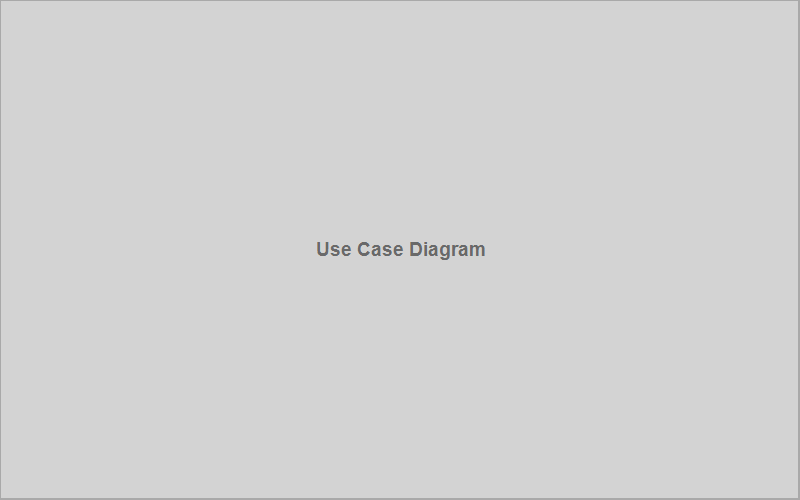
\includegraphics[width=0.9\textwidth]{assets/diagrams/usecase_diagram.png}
    \caption{Biểu đồ ca sử dụng tổng quan hệ thống SmartNutri}
    \label{fig:usecase_diagram}
\end{figure}

\section{Mô tả ca sử dụng}

% ============================================================
\subsection{UC-01: Đăng ký tài khoản}

\begin{longtable}{|p{4cm}|p{11cm}|}
    \hline
    \textbf{Thuộc tính} & \textbf{Mô tả} \\
    \hline
    \endhead
    \hline
    \endfoot
    Tên ca sử dụng & Đăng ký tài khoản \\
    \hline
    Mô tả & Người dùng tạo tài khoản mới để sử dụng ứng dụng. \\
    \hline
    Actor & Người dùng (chưa có tài khoản) \\
    \hline
    Luồng cơ bản &
        \begin{enumerate}[nosep]
            \item Người dùng mở ứng dụng, chọn ``Đăng ký''.
            \item Hệ thống hiển thị form đăng ký (email, mật khẩu, xác nhận mật khẩu).
            \item Người dùng nhập thông tin và nhấn ``Đăng ký''.
            \item Hệ thống kiểm tra tính hợp lệ của dữ liệu.
            \item Firebase Auth tạo tài khoản mới và gửi email xác minh.
            \item Hệ thống tạo document người dùng trong Firestore.
            \item Hệ thống chuyển đến màn hình Onboarding.
        \end{enumerate} \\
    \hline
    Luồng thay thế &
        \begin{enumerate}[nosep]
            \item[3a.] Email đã tồn tại: Hiển thị thông báo lỗi ``Email đã được sử dụng''.
            \item[3b.] Mật khẩu không đủ mạnh: Yêu cầu mật khẩu tối thiểu 6 ký tự.
            \item[3c.] Mất kết nối mạng: Hiển thị thông báo lỗi kết nối.
        \end{enumerate} \\
    \hline
    Tiền điều kiện & Người dùng chưa có tài khoản trong hệ thống. \\
    \hline
    Hậu điều kiện & Tài khoản được tạo, document người dùng được lưu trong Firestore, email xác minh được gửi. \\
    \hline
    Business Rules &
        \begin{itemize}[nosep]
            \item Email phải đúng định dạng.
            \item Mật khẩu tối thiểu 6 ký tự.
            \item Mỗi email chỉ được đăng ký một tài khoản.
        \end{itemize} \\
    \hline
\end{longtable}

\begin{figure}[H]
    \centering
    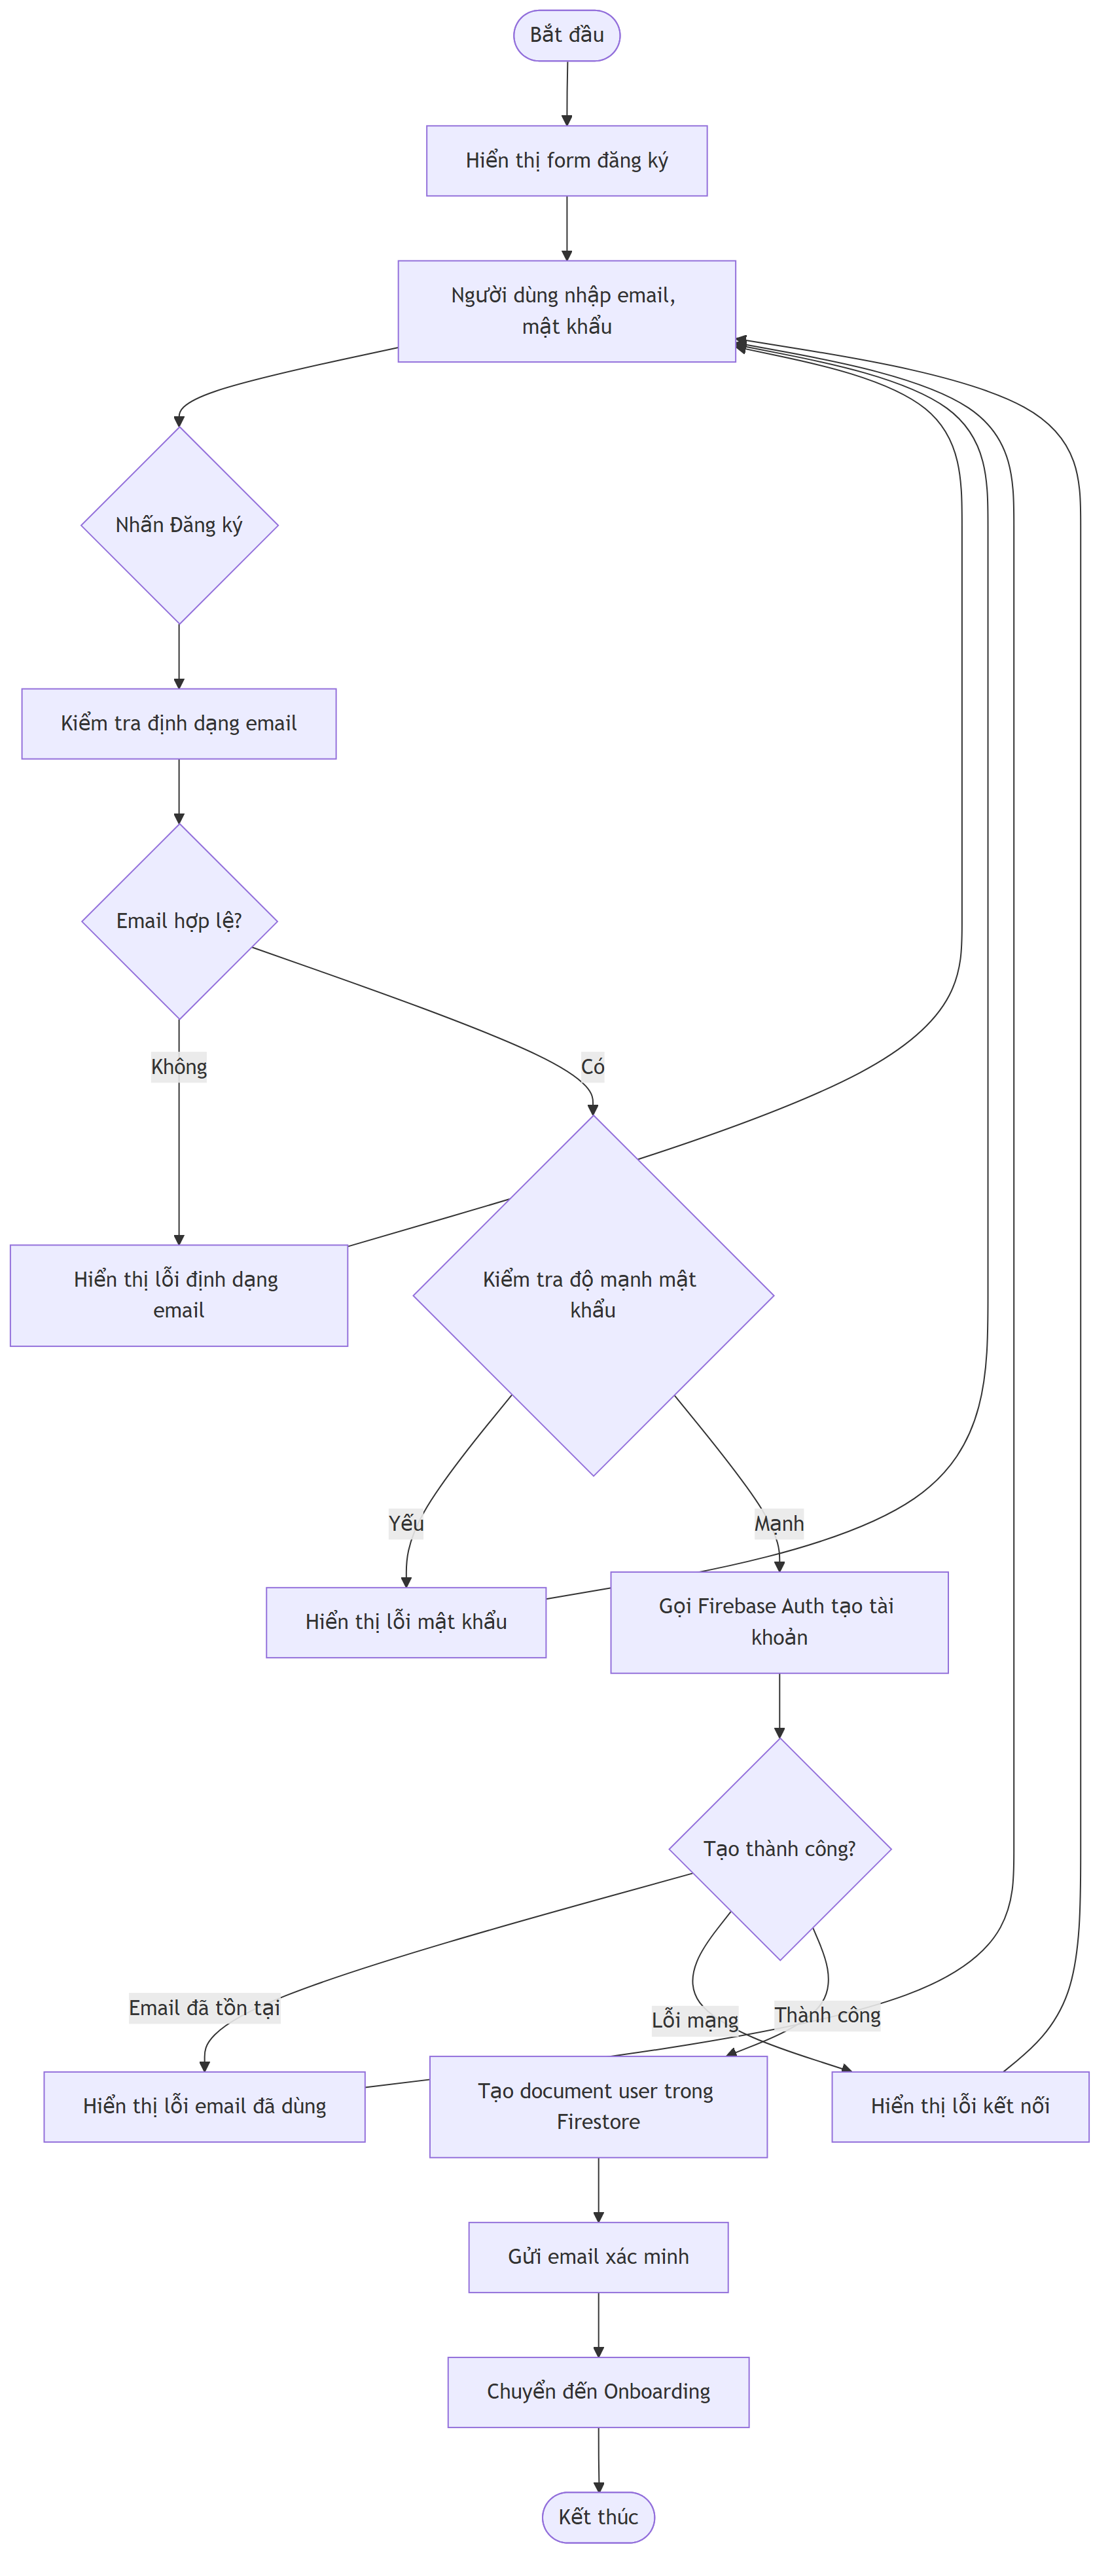
\includegraphics[width=0.8\textwidth]{assets/diagrams/uc01_register_activity.png}
    \caption{Biểu đồ hoạt động ca sử dụng Đăng ký tài khoản}
    \label{fig:uc01_register_activity}
\end{figure}

\begin{figure}[H]
    \centering
    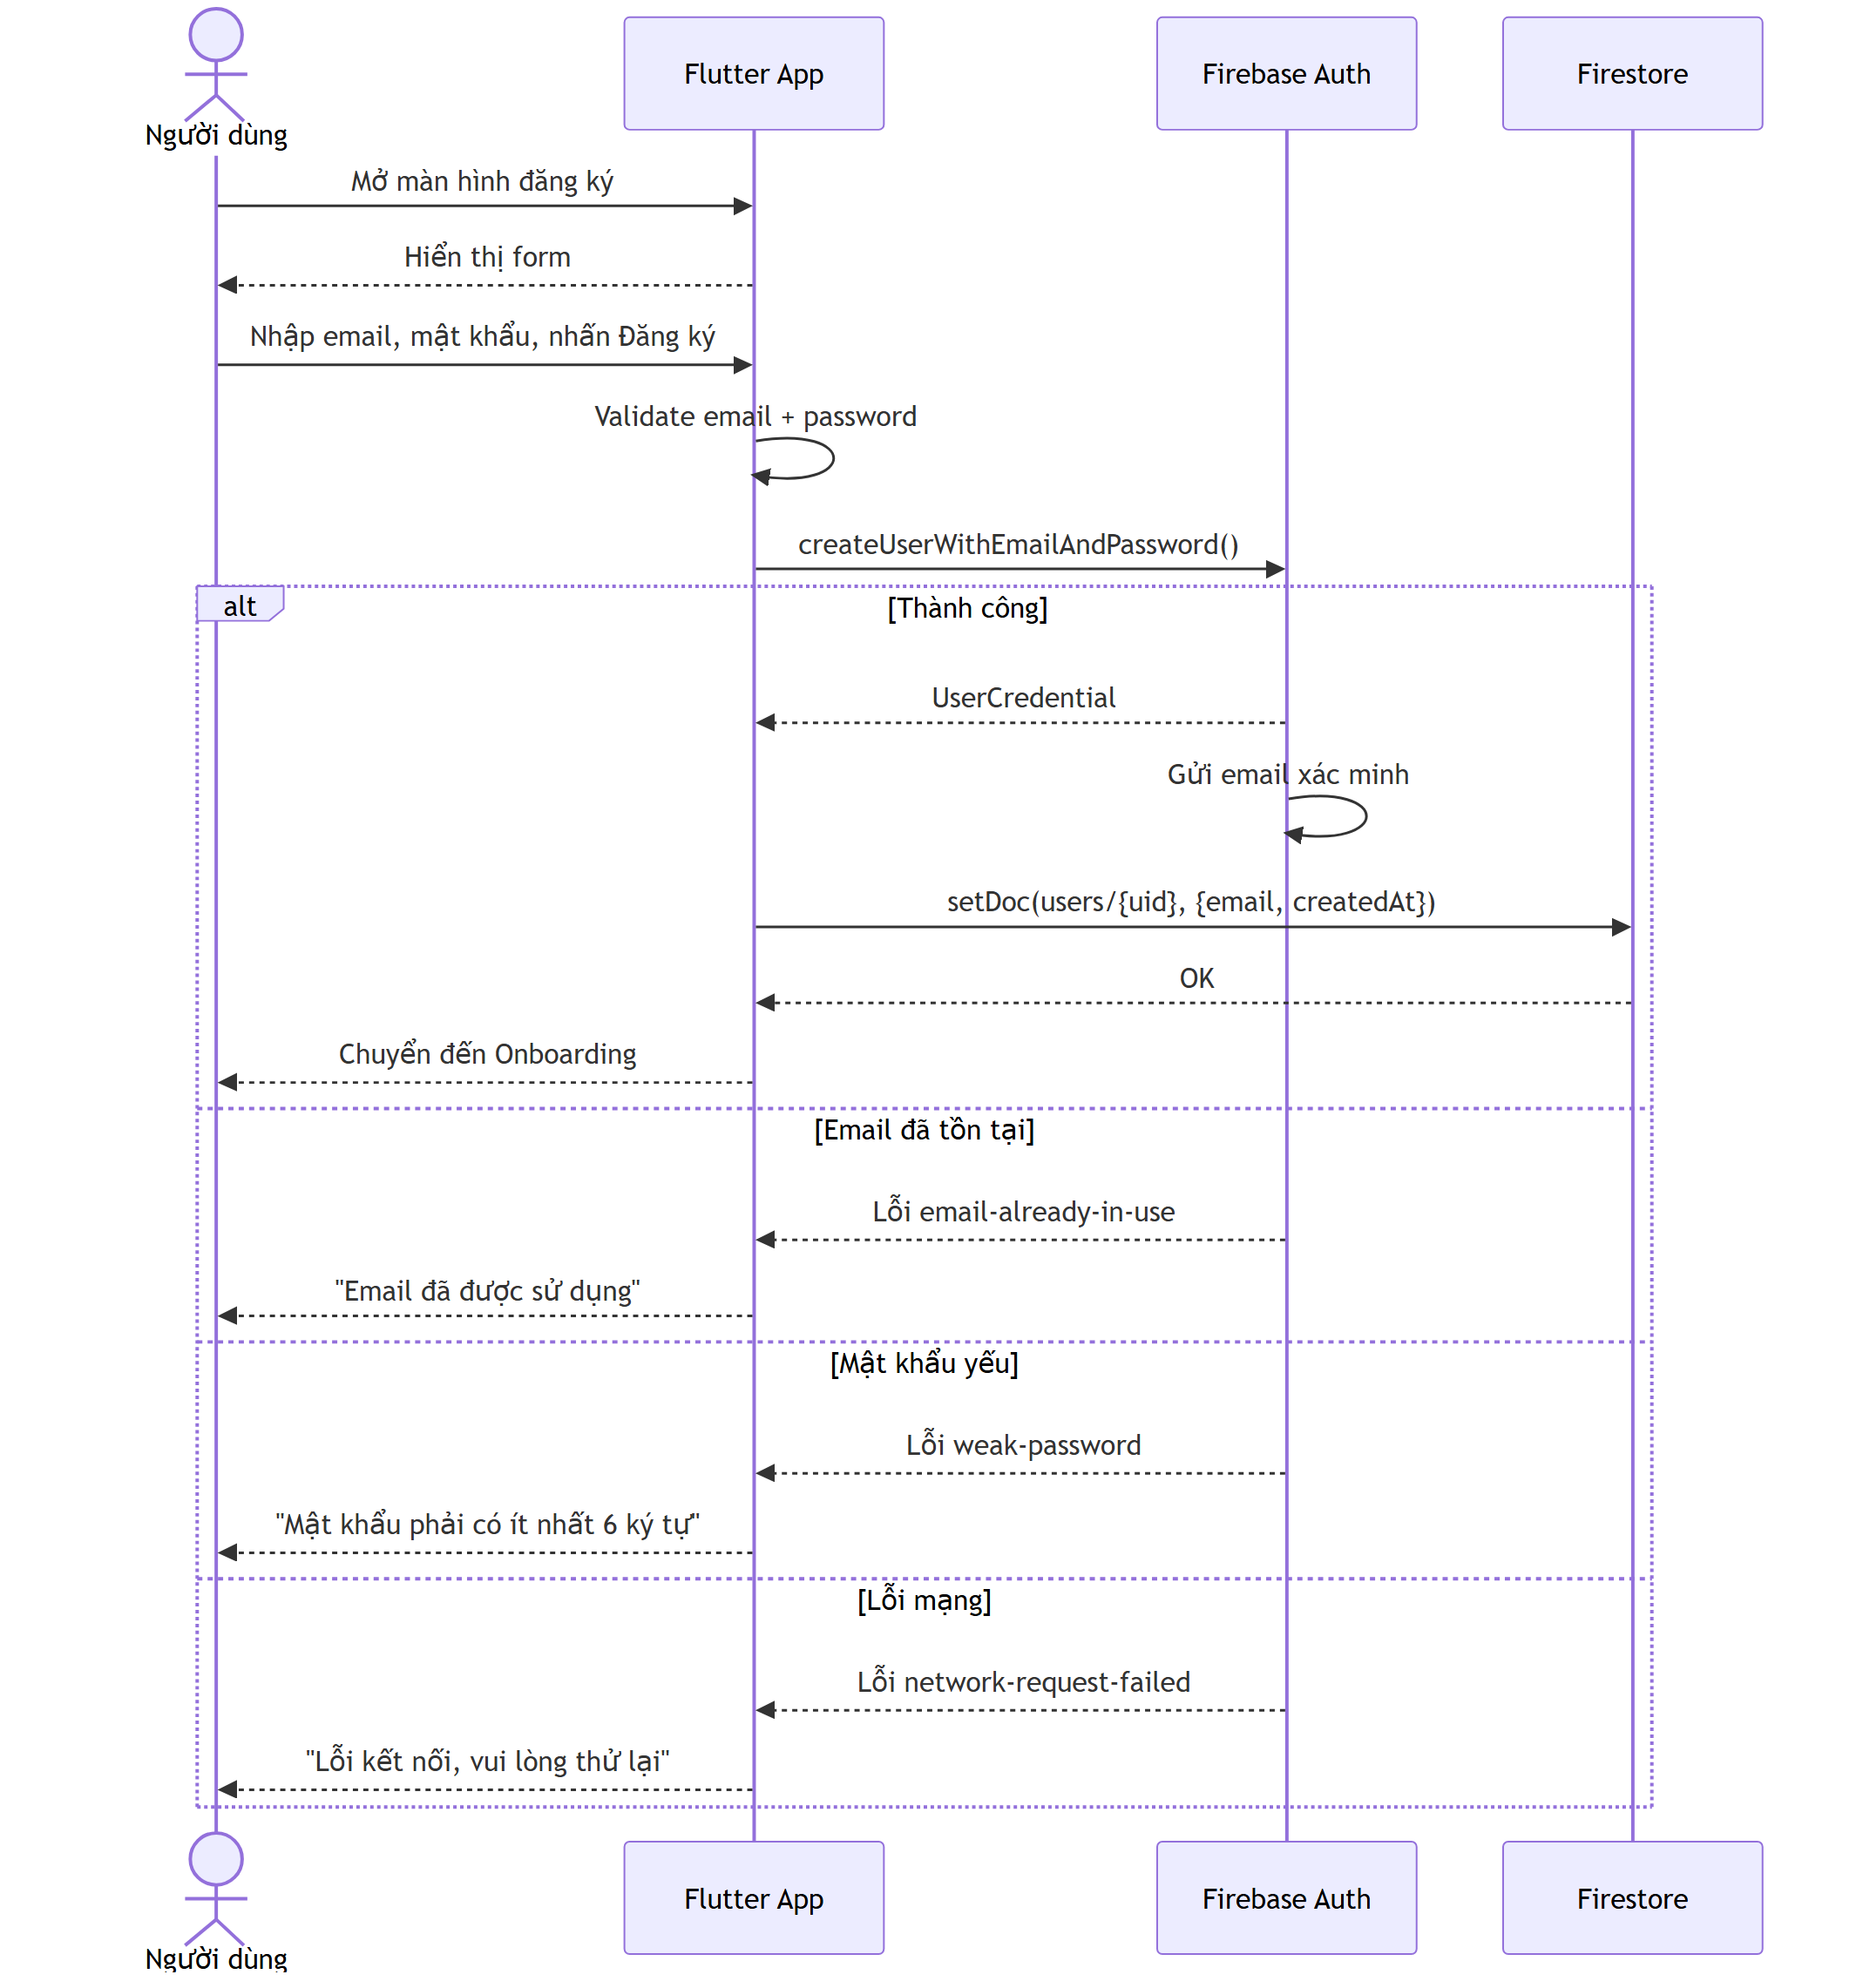
\includegraphics[width=0.9\textwidth]{assets/diagrams/uc01_register_sequence.png}
    \caption{Biểu đồ tuần tự ca sử dụng Đăng ký tài khoản}
    \label{fig:uc01_register_sequence}
\end{figure}

% ============================================================
\subsection{UC-02: Đăng nhập}

\begin{longtable}{|p{4cm}|p{11cm}|}
    \hline
    \textbf{Thuộc tính} & \textbf{Mô tả} \\
    \hline
    \endhead
    \hline
    \endfoot
    Tên ca sử dụng & Đăng nhập \\
    \hline
    Mô tả & Người dùng đăng nhập vào hệ thống để truy cập các chức năng cá nhân hóa như nhật ký ăn uống, thống kê dinh dưỡng và chatbot AI. \\
    \hline
    Actor & Người dùng đã có tài khoản \\
    \hline
    Luồng cơ bản &
        \begin{enumerate}[nosep]
            \item Người dùng mở ứng dụng và chọn chức năng đăng nhập.
            \item Hệ thống hiển thị form đăng nhập.
            \item Người dùng nhập email và mật khẩu, sau đó nhấn ``Đăng nhập''.
            \item Hệ thống gửi thông tin xác thực đến Firebase Authentication.
            \item Firebase Authentication xác thực thông tin đăng nhập.
            \item Hệ thống tải thông tin hồ sơ người dùng từ Firestore.
            \item Hệ thống chuyển người dùng đến màn hình chính.
        \end{enumerate} \\
    \hline
    Luồng thay thế &
        \begin{enumerate}[nosep]
            \item[3a.] Người dùng chọn đăng nhập bằng Google: Hệ thống mở màn hình chọn tài khoản Google, sau đó xác thực qua Firebase Authentication.
            \item[4a.] Email hoặc mật khẩu không hợp lệ: Hệ thống hiển thị thông báo lỗi và cho phép nhập lại.
            \item[6a.] Hồ sơ người dùng chưa hoàn tất: Hệ thống chuyển người dùng đến màn hình Onboarding.
        \end{enumerate} \\
    \hline
    Tiền điều kiện & Người dùng đã có tài khoản trong hệ thống. \\
    \hline
    Hậu điều kiện & Người dùng được xác thực và có thể truy cập các chức năng chính của ứng dụng. \\
    \hline
    Business Rules &
        \begin{itemize}[nosep]
            \item Không cho phép truy cập dữ liệu cá nhân nếu người dùng chưa đăng nhập.
            \item Thông tin xác thực được xử lý qua Firebase Authentication.
            \item Nếu hồ sơ chưa hoàn tất, người dùng phải hoàn thành Onboarding trước khi dùng đầy đủ chức năng.
        \end{itemize} \\
    \hline
\end{longtable}

\begin{figure}[H]
    \centering
    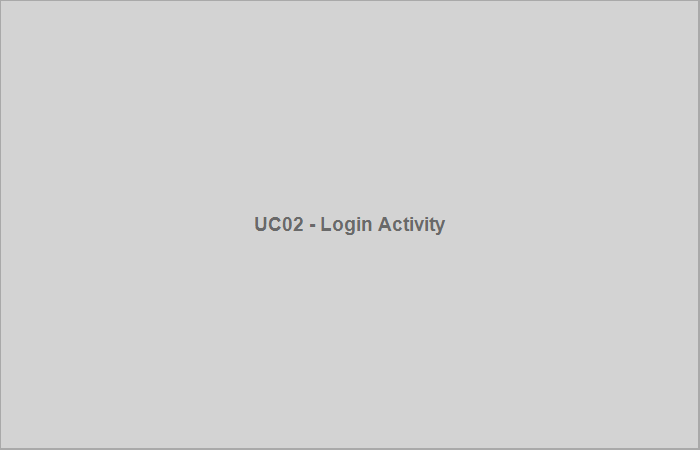
\includegraphics[width=0.8\textwidth]{assets/diagrams/uc02_login_activity.png}
    \caption{Biểu đồ hoạt động ca sử dụng Đăng nhập}
    \label{fig:uc02_login_activity}
\end{figure}

\begin{figure}[H]
    \centering
    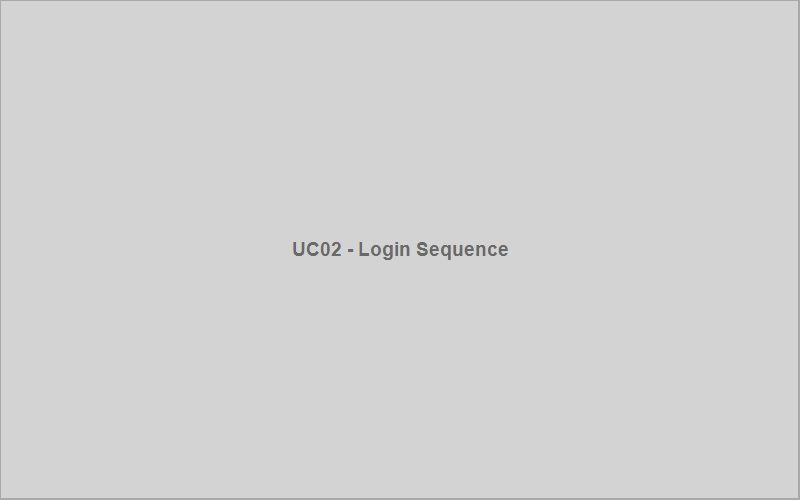
\includegraphics[width=0.9\textwidth]{assets/diagrams/uc02_login_sequence.png}
    \caption{Biểu đồ tuần tự ca sử dụng Đăng nhập}
    \label{fig:uc02_login_sequence}
\end{figure}

% ============================================================
\subsection{UC-05: Quét món ăn bằng AI}

\begin{longtable}{|p{4cm}|p{11cm}|}
    \hline
    \textbf{Thuộc tính} & \textbf{Mô tả} \\
    \hline
    \endhead
    \hline
    \endfoot
    Tên ca sử dụng & Quét món ăn bằng AI \\
    \hline
    Mô tả & Người dùng chụp ảnh hoặc tải ảnh món ăn lên; hệ thống sử dụng AI để nhận diện món ăn và trả về thông tin dinh dưỡng. \\
    \hline
    Actor & Người dùng (đã đăng nhập) \\
    \hline
    Luồng cơ bản &
        \begin{enumerate}[nosep]
            \item Người dùng nhấn nút ``Scan'' trên màn hình chính.
            \item Hệ thống mở camera hoặc cho phép chọn ảnh từ thư viện.
            \item Người dùng chụp ảnh hoặc chọn ảnh món ăn.
            \item Hệ thống gửi ảnh đến Cloud Function ``scanFood''.
            \item Cloud Function gọi Gemini API để phân tích ảnh.
            \item Gemini trả về tên món ăn và thông tin dinh dưỡng ước tính.
            \item Hệ thống hiển thị kết quả nhận diện cho người dùng.
            \item Người dùng xác nhận và thêm món ăn vào nhật ký.
        \end{enumerate} \\
    \hline
    Luồng thay thế &
        \begin{enumerate}[nosep]
            \item[5a.] Gemini không nhận diện được món ăn: Hiển thị ``Không thể nhận diện món ăn, vui lòng thử lại''.
            \item[5b.] Gemini API lỗi/quá tải: Fallback về xử lý trực tiếp từ client với cấu hình đơn giản hơn.
            \item[5c.] Người dùng hủy thao tác: Quay về màn hình chính.
        \end{enumerate} \\
    \hline
    Tiền điều kiện & Người dùng đã đăng nhập, thiết bị có kết nối mạng. \\
    \hline
    Hậu điều kiện & Món ăn được thêm vào nhật ký dinh dưỡng của người dùng trong ngày. \\
    \hline
    Business Rules &
        \begin{itemize}[nosep]
            \item Ảnh phải có độ phân giải tối thiểu 224x224 pixels.
            \item Kết quả dinh dưỡng từ AI là ước tính, người dùng có thể chỉnh sửa.
            \item Chỉ hỗ trợ nhận diện món ăn Việt Nam và phổ biến.
        \end{itemize} \\
    \hline
\end{longtable}

\begin{figure}[H]
    \centering
    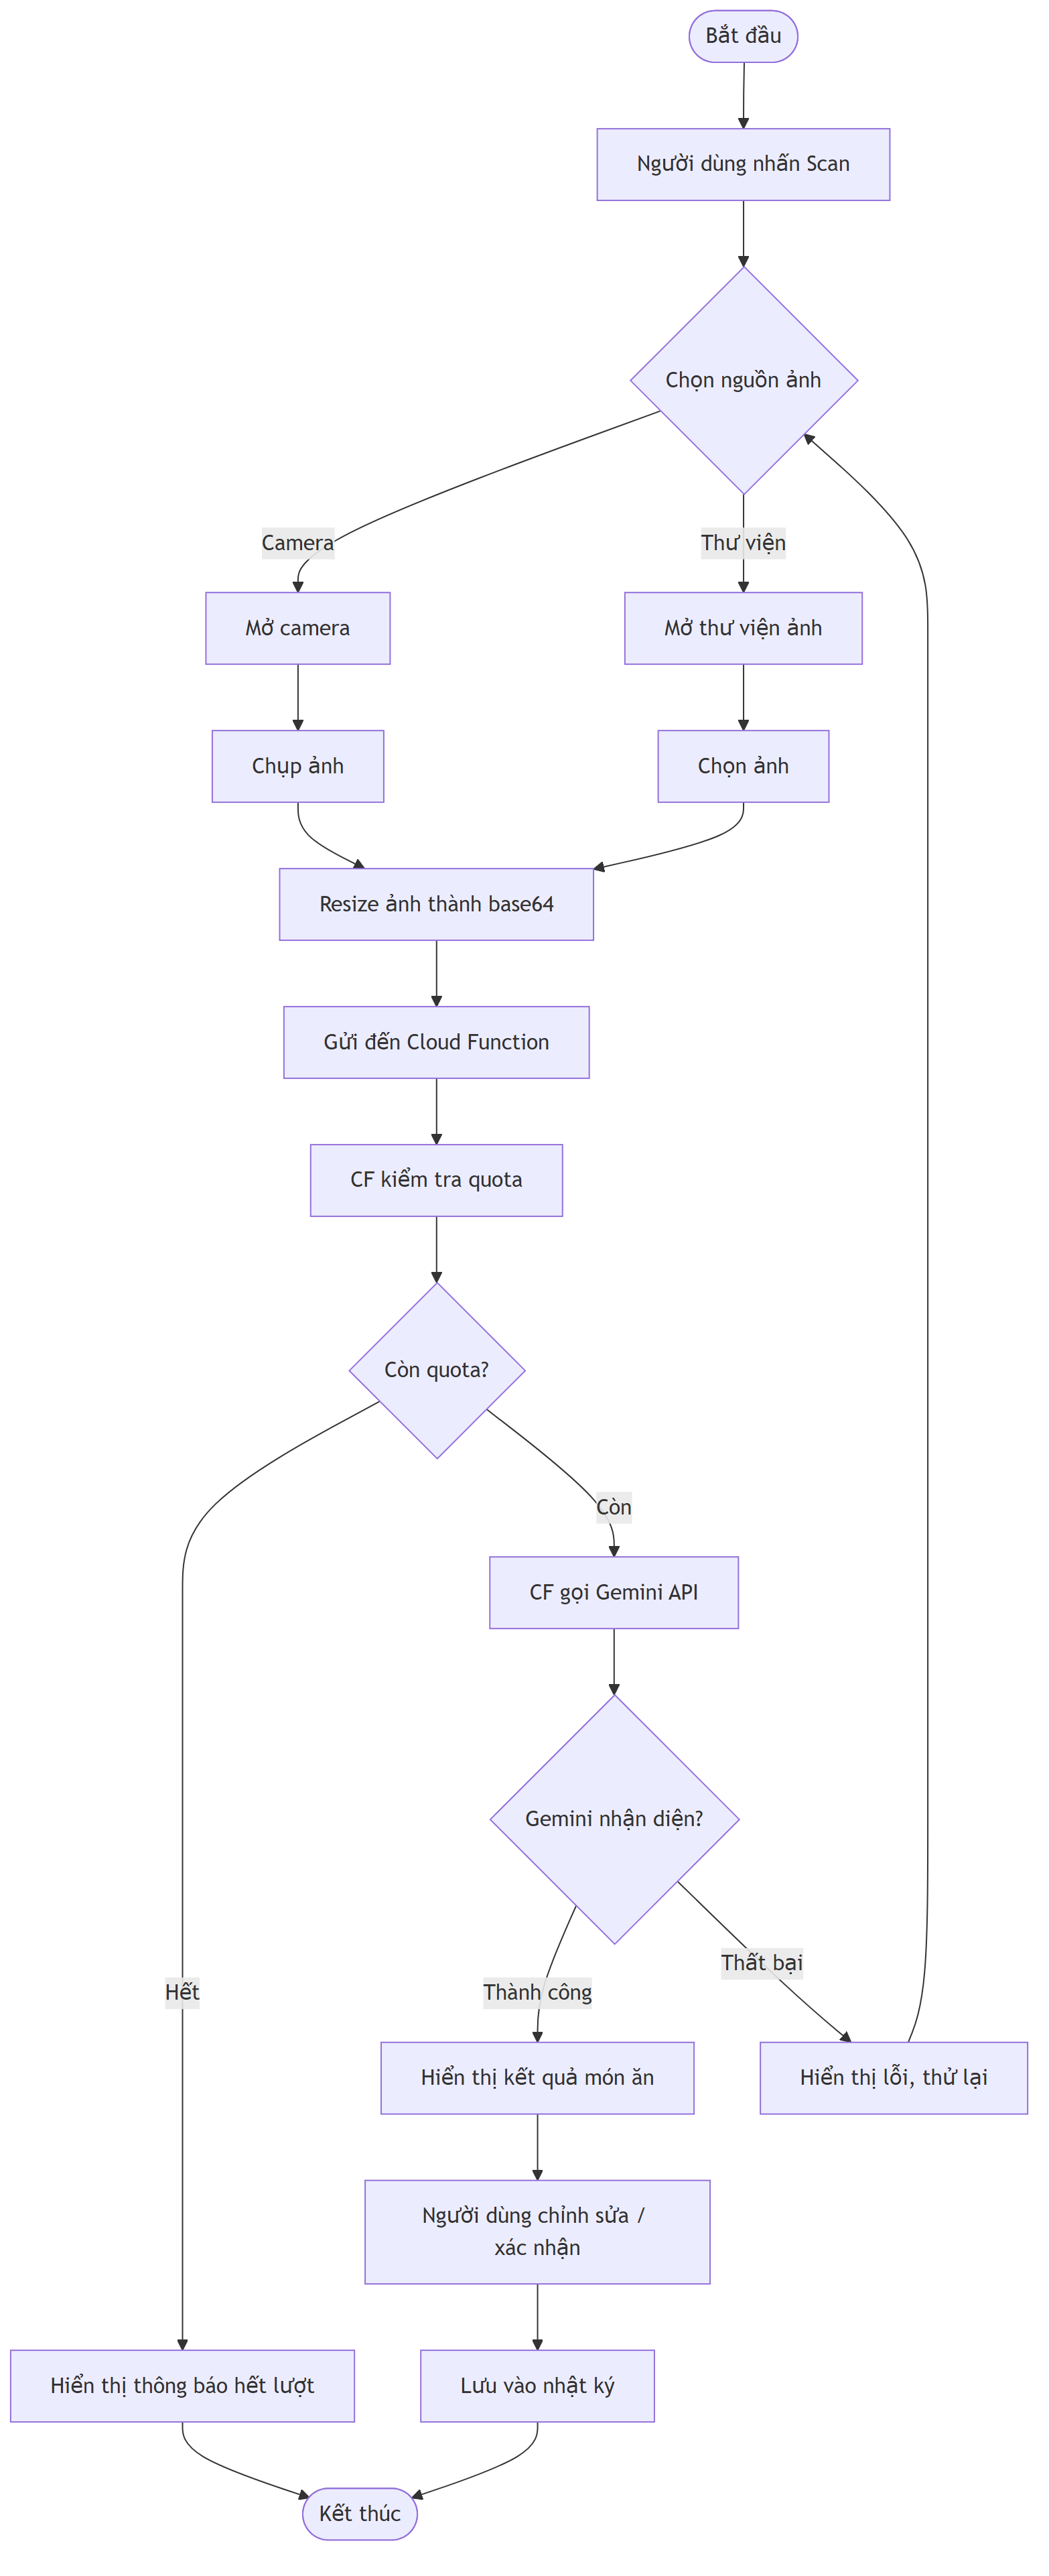
\includegraphics[width=0.8\textwidth]{assets/diagrams/uc05_scan_activity.png}
    \caption{Biểu đồ hoạt động ca sử dụng Quét món ăn bằng AI}
    \label{fig:uc05_scan_activity}
\end{figure}

\begin{figure}[H]
    \centering
    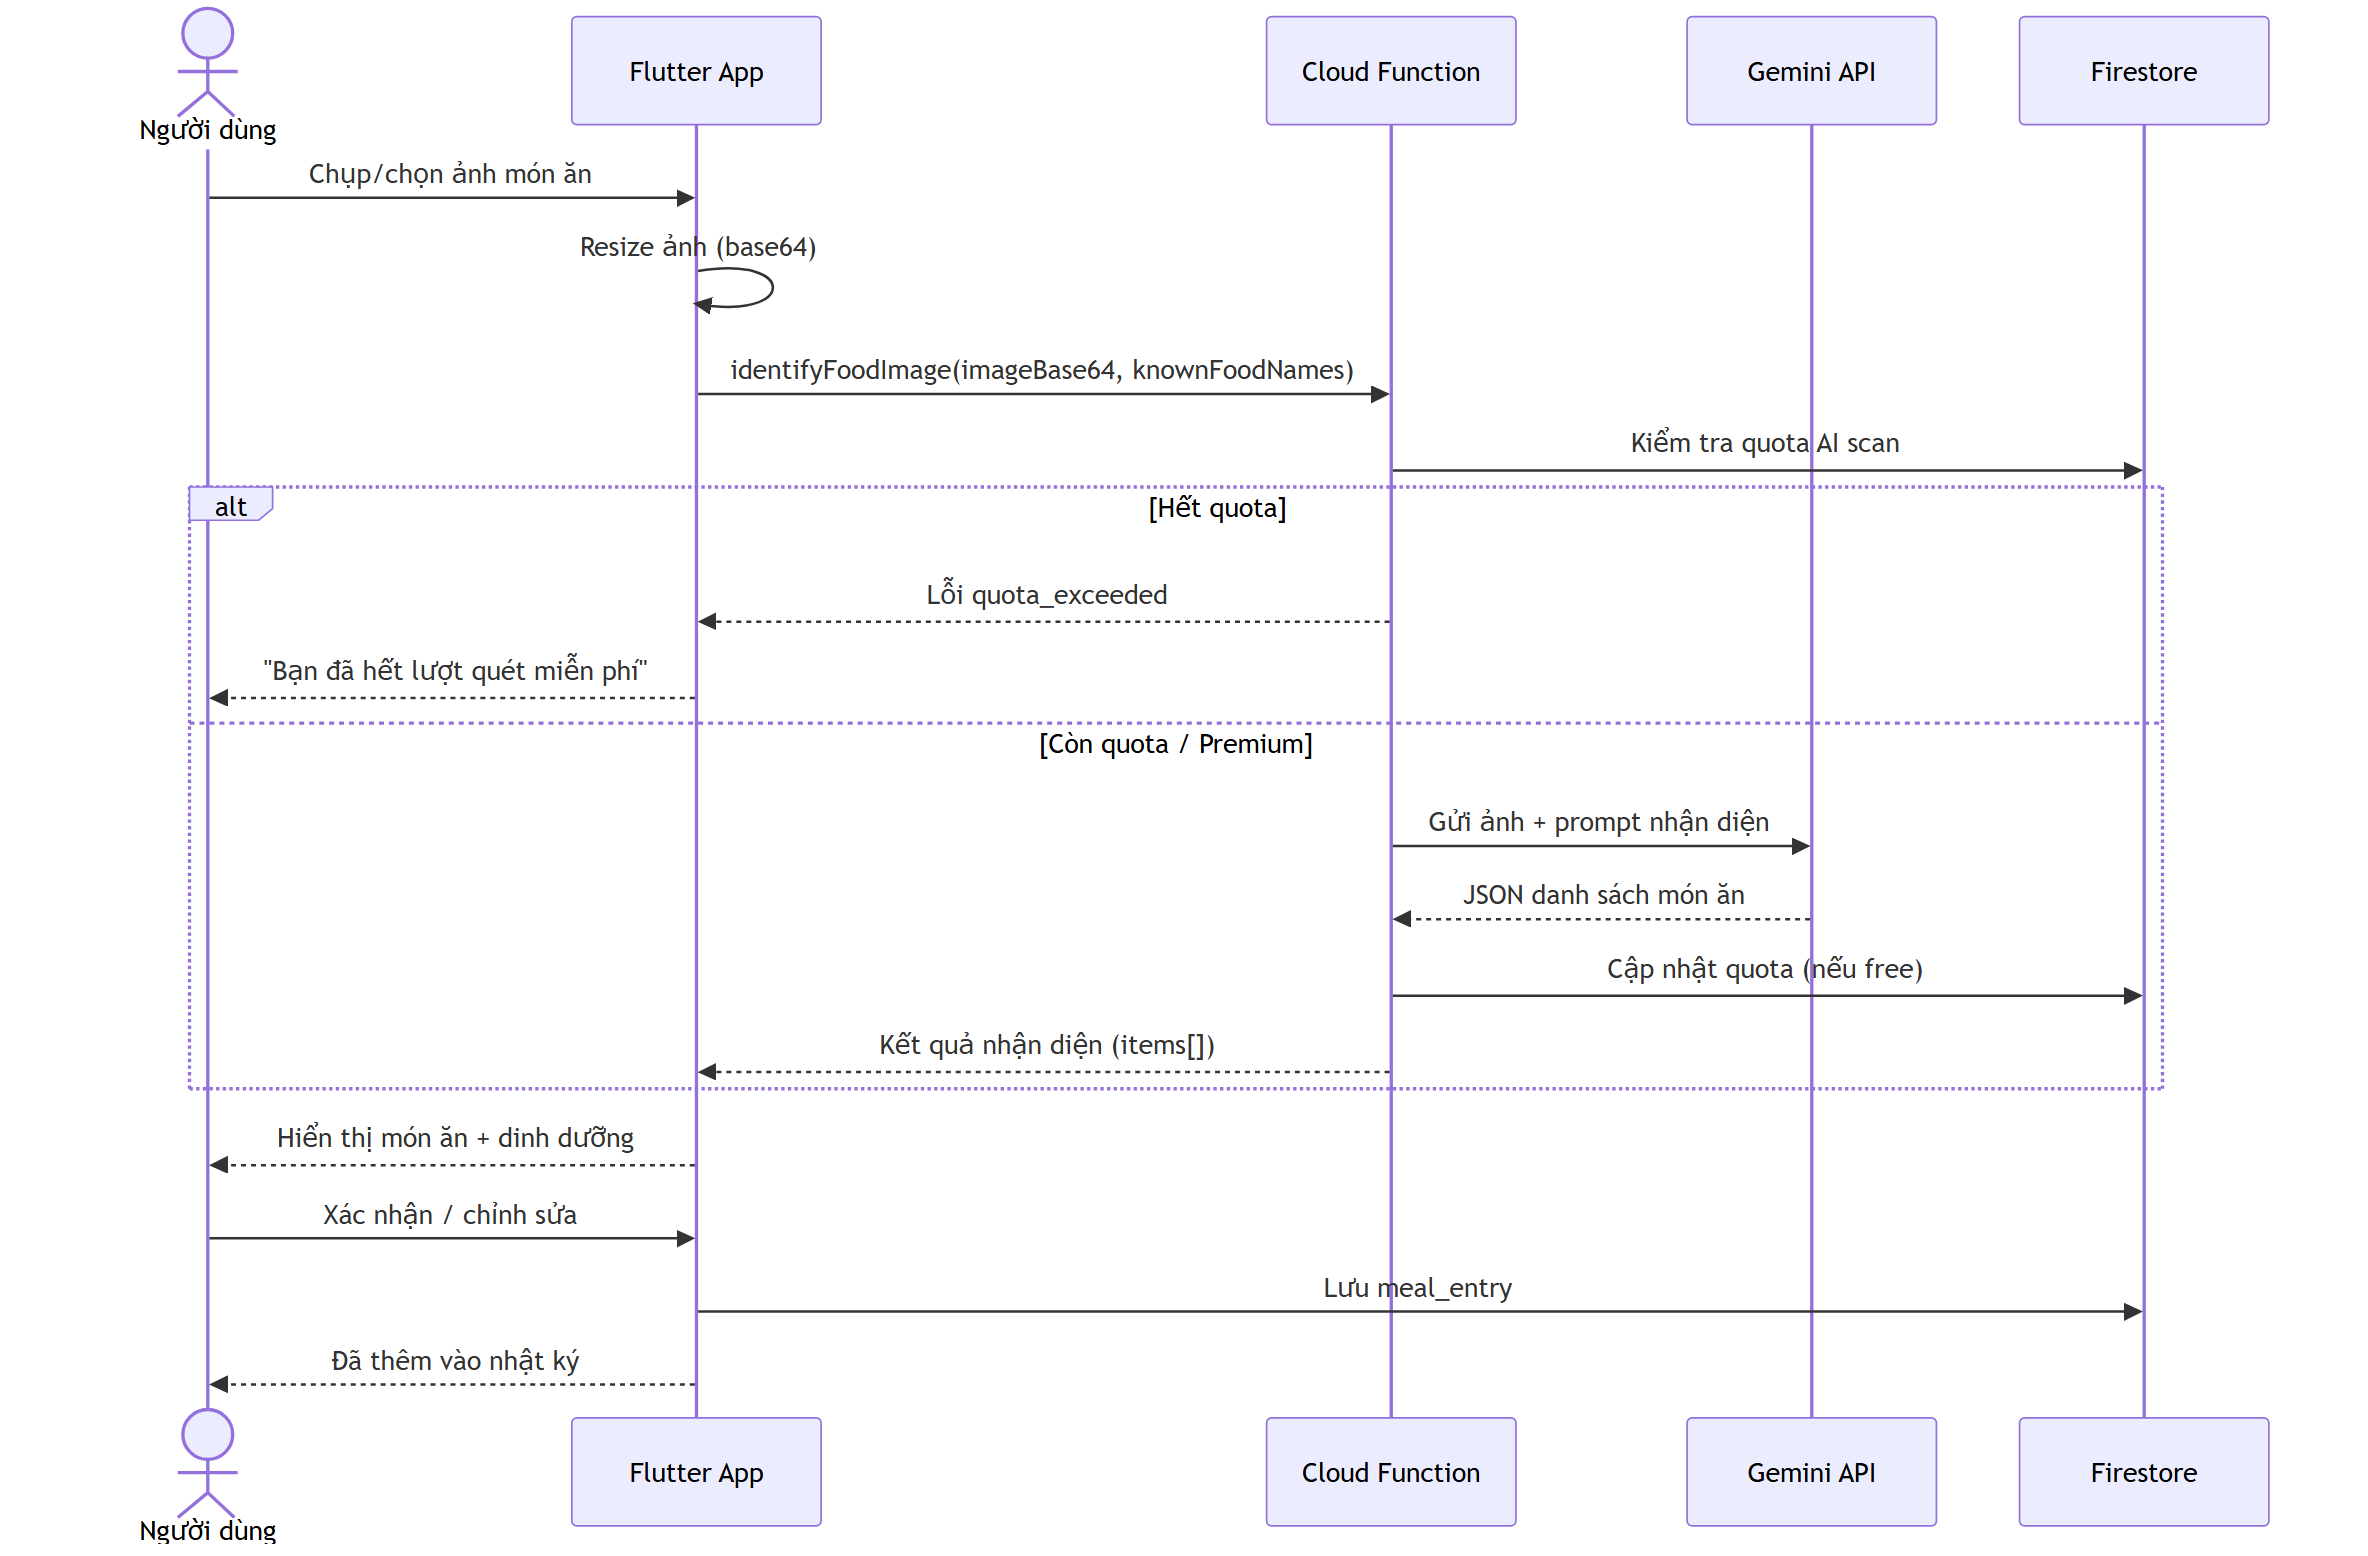
\includegraphics[width=0.9\textwidth]{assets/diagrams/uc05_scan_sequence.png}
    \caption{Biểu đồ tuần tự ca sử dụng Quét món ăn bằng AI}
    \label{fig:uc05_scan_sequence}
\end{figure}

% ============================================================
\subsection{UC-06: Nhật ký ăn uống}

\begin{longtable}{|p{4cm}|p{11cm}|}
    \hline
    \textbf{Thuộc tính} & \textbf{Mô tả} \\
    \hline
    \endhead
    \hline
    \endfoot
    Tên ca sử dụng & Nhật ký ăn uống \\
    \hline
    Mô tả & Người dùng xem, thêm, chỉnh sửa hoặc xóa các món ăn đã ghi nhận trong ngày để theo dõi lượng dinh dưỡng tiêu thụ. \\
    \hline
    Actor & Người dùng đã đăng nhập \\
    \hline
    Luồng cơ bản &
        \begin{enumerate}[nosep]
            \item Người dùng mở màn hình nhật ký ăn uống.
            \item Hệ thống truy xuất danh sách món ăn đã ghi nhận trong ngày từ Firestore.
            \item Hệ thống hiển thị danh sách món ăn theo từng bữa: sáng, trưa, tối và bữa phụ.
            \item Người dùng chọn thêm món ăn thủ công hoặc thêm từ kết quả quét AI.
            \item Người dùng nhập khẩu phần hoặc điều chỉnh thông tin dinh dưỡng nếu cần.
            \item Hệ thống lưu bản ghi mới vào sub-collection nhật ký của người dùng.
            \item Hệ thống cập nhật tổng calo và các chỉ số dinh dưỡng trong ngày.
        \end{enumerate} \\
    \hline
    Luồng thay thế &
        \begin{enumerate}[nosep]
            \item[2a.] Không có dữ liệu trong ngày: Hệ thống hiển thị trạng thái rỗng và gợi ý người dùng thêm món ăn.
            \item[5a.] Người dùng hủy thao tác thêm món: Hệ thống quay lại danh sách nhật ký hiện tại.
            \item[6a.] Lưu dữ liệu thất bại do mất mạng: Hệ thống hiển thị thông báo lỗi và cho phép thử lại.
        \end{enumerate} \\
    \hline
    Tiền điều kiện & Người dùng đã đăng nhập và có quyền truy cập dữ liệu cá nhân của mình. \\
    \hline
    Hậu điều kiện & Nhật ký ăn uống được cập nhật, tổng dinh dưỡng trong ngày được tính lại. \\
    \hline
    Business Rules &
        \begin{itemize}[nosep]
            \item Mỗi bản ghi nhật ký thuộc về đúng một người dùng.
            \item Người dùng chỉ được chỉnh sửa hoặc xóa bản ghi của chính mình.
            \item Thông tin dinh dưỡng được tính theo khẩu phần thực tế đã nhập.
        \end{itemize} \\
    \hline
\end{longtable}

\begin{figure}[H]
    \centering
    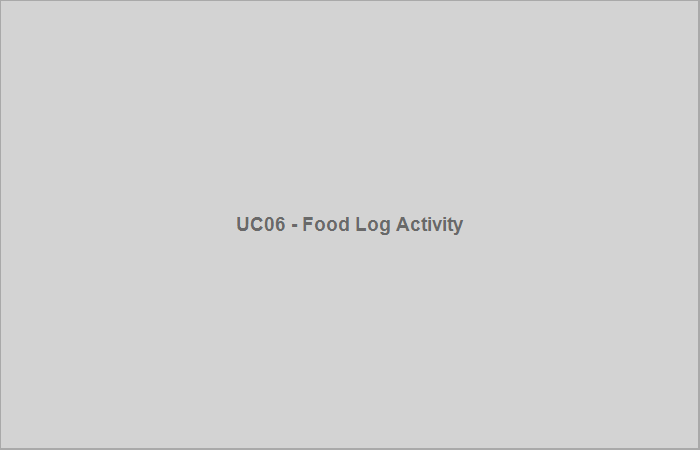
\includegraphics[width=0.8\textwidth]{assets/diagrams/uc06_foodlog_activity.png}
    \caption{Biểu đồ hoạt động ca sử dụng Nhật ký ăn uống}
    \label{fig:uc06_foodlog_activity}
\end{figure}

\begin{figure}[H]
    \centering
    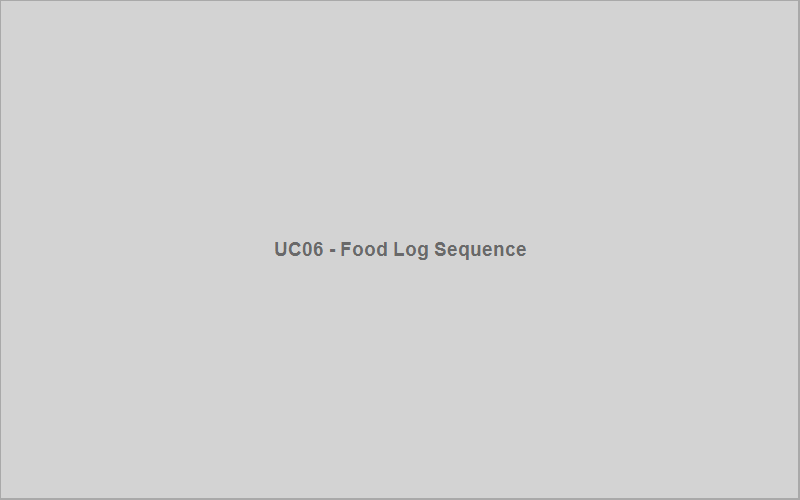
\includegraphics[width=0.9\textwidth]{assets/diagrams/uc06_foodlog_sequence.png}
    \caption{Biểu đồ tuần tự ca sử dụng Nhật ký ăn uống}
    \label{fig:uc06_foodlog_sequence}
\end{figure}

% ============================================================
\subsection{UC-07: Theo dõi dinh dưỡng}

\begin{longtable}{|p{4cm}|p{11cm}|}
    \hline
    \textbf{Thuộc tính} & \textbf{Mô tả} \\
    \hline
    \endhead
    \hline
    \endfoot
    Tên ca sử dụng & Theo dõi dinh dưỡng \\
    \hline
    Mô tả & Người dùng xem tổng quan lượng calo và các nhóm chất dinh dưỡng đã tiêu thụ, từ đó so sánh với mục tiêu cá nhân. \\
    \hline
    Actor & Người dùng đã đăng nhập \\
    \hline
    Luồng cơ bản &
        \begin{enumerate}[nosep]
            \item Người dùng mở màn hình thống kê dinh dưỡng.
            \item Hệ thống truy xuất nhật ký ăn uống theo khoảng thời gian được chọn.
            \item Hệ thống tính tổng calo, protein, carbohydrate và chất béo.
            \item Hệ thống so sánh kết quả với mục tiêu dinh dưỡng của người dùng.
            \item Hệ thống hiển thị biểu đồ và thẻ thống kê tổng quan.
            \item Người dùng chuyển đổi giữa chế độ xem ngày, tuần hoặc tháng.
        \end{enumerate} \\
    \hline
    Luồng thay thế &
        \begin{enumerate}[nosep]
            \item[2a.] Không có dữ liệu trong khoảng thời gian được chọn: Hệ thống hiển thị thông báo chưa có dữ liệu.
            \item[4a.] Người dùng chưa thiết lập mục tiêu dinh dưỡng: Hệ thống hiển thị số liệu tiêu thụ và gợi ý hoàn thiện hồ sơ.
            \item[6a.] Người dùng chọn khoảng thời gian khác: Hệ thống tải lại dữ liệu tương ứng.
        \end{enumerate} \\
    \hline
    Tiền điều kiện & Người dùng đã đăng nhập; dữ liệu nhật ký ăn uống có thể tồn tại hoặc chưa tồn tại. \\
    \hline
    Hậu điều kiện & Người dùng nắm được tình trạng tiêu thụ dinh dưỡng so với mục tiêu cá nhân. \\
    \hline
    Business Rules &
        \begin{itemize}[nosep]
            \item Số liệu thống kê chỉ tính từ dữ liệu nhật ký của người dùng hiện tại.
            \item Các chỉ số macro bao gồm protein, carbohydrate và chất béo.
            \item Nếu dữ liệu thiếu hoặc chưa đủ, hệ thống phải thể hiện rõ trạng thái chưa có dữ liệu thay vì suy đoán.
        \end{itemize} \\
    \hline
\end{longtable}

\begin{figure}[H]
    \centering
    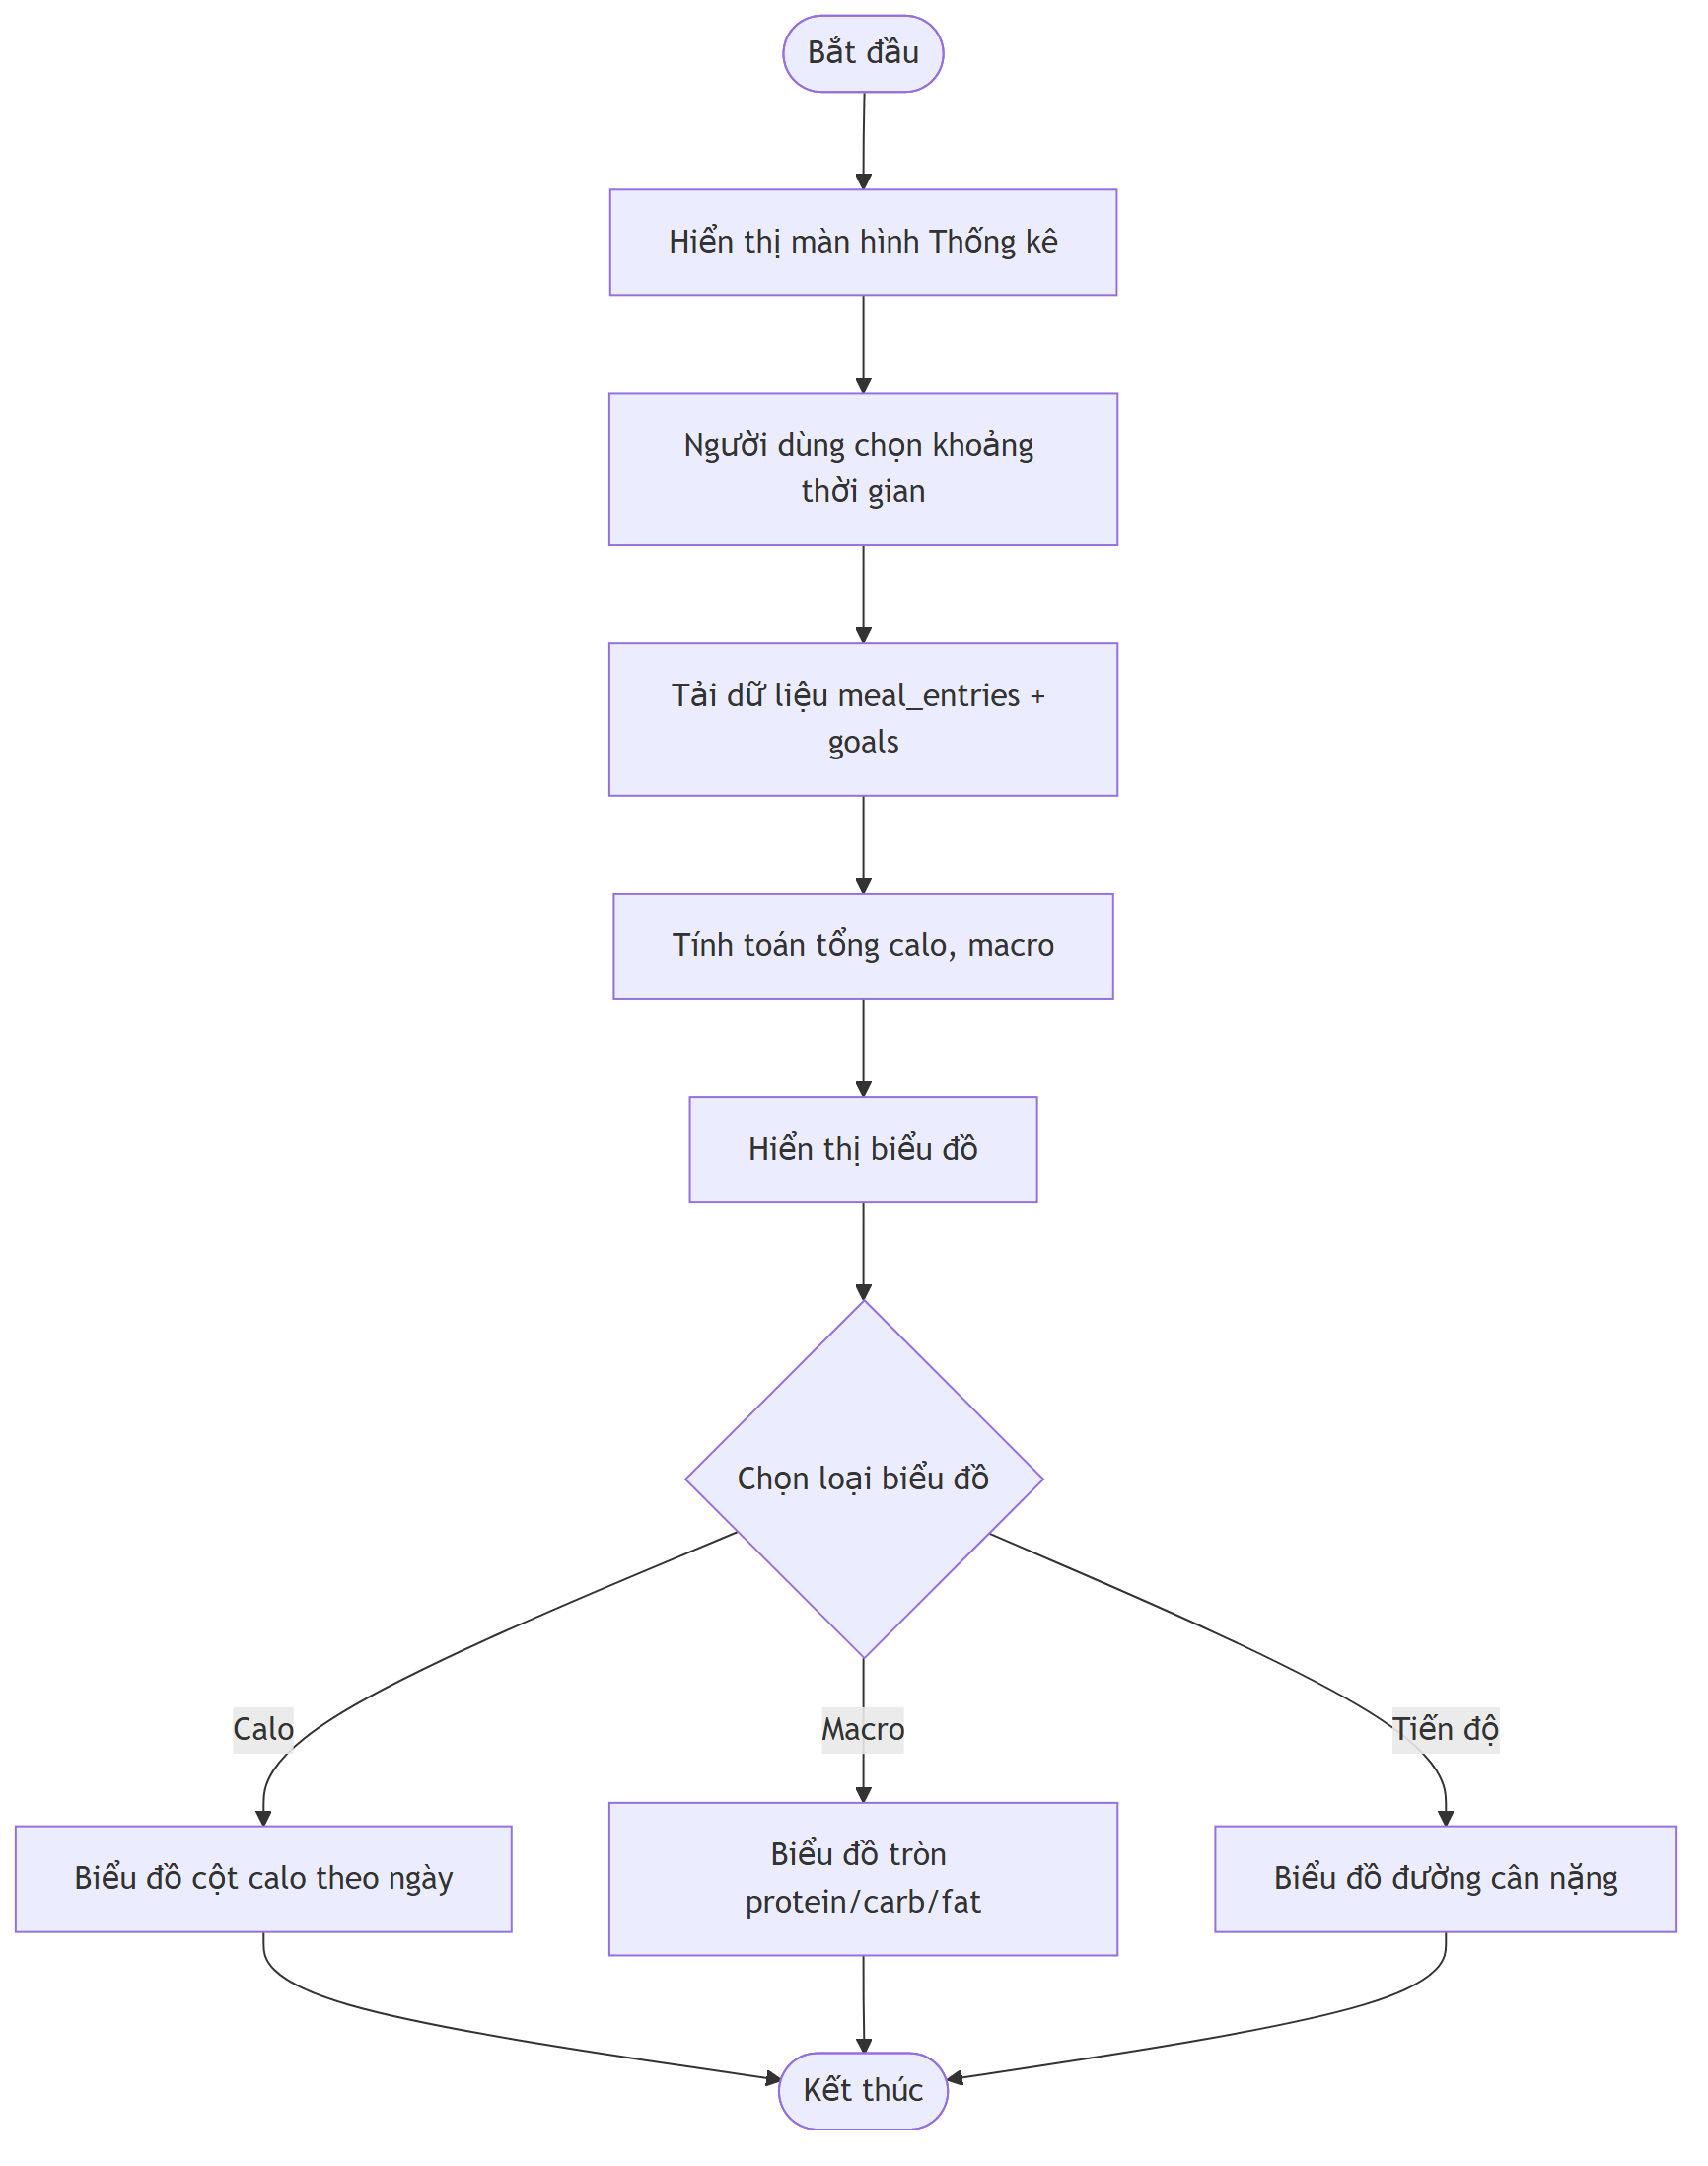
\includegraphics[width=0.8\textwidth]{assets/diagrams/uc07_stats_activity.png}
    \caption{Biểu đồ hoạt động ca sử dụng Theo dõi dinh dưỡng}
    \label{fig:uc07_stats_activity}
\end{figure}

\begin{figure}[H]
    \centering
    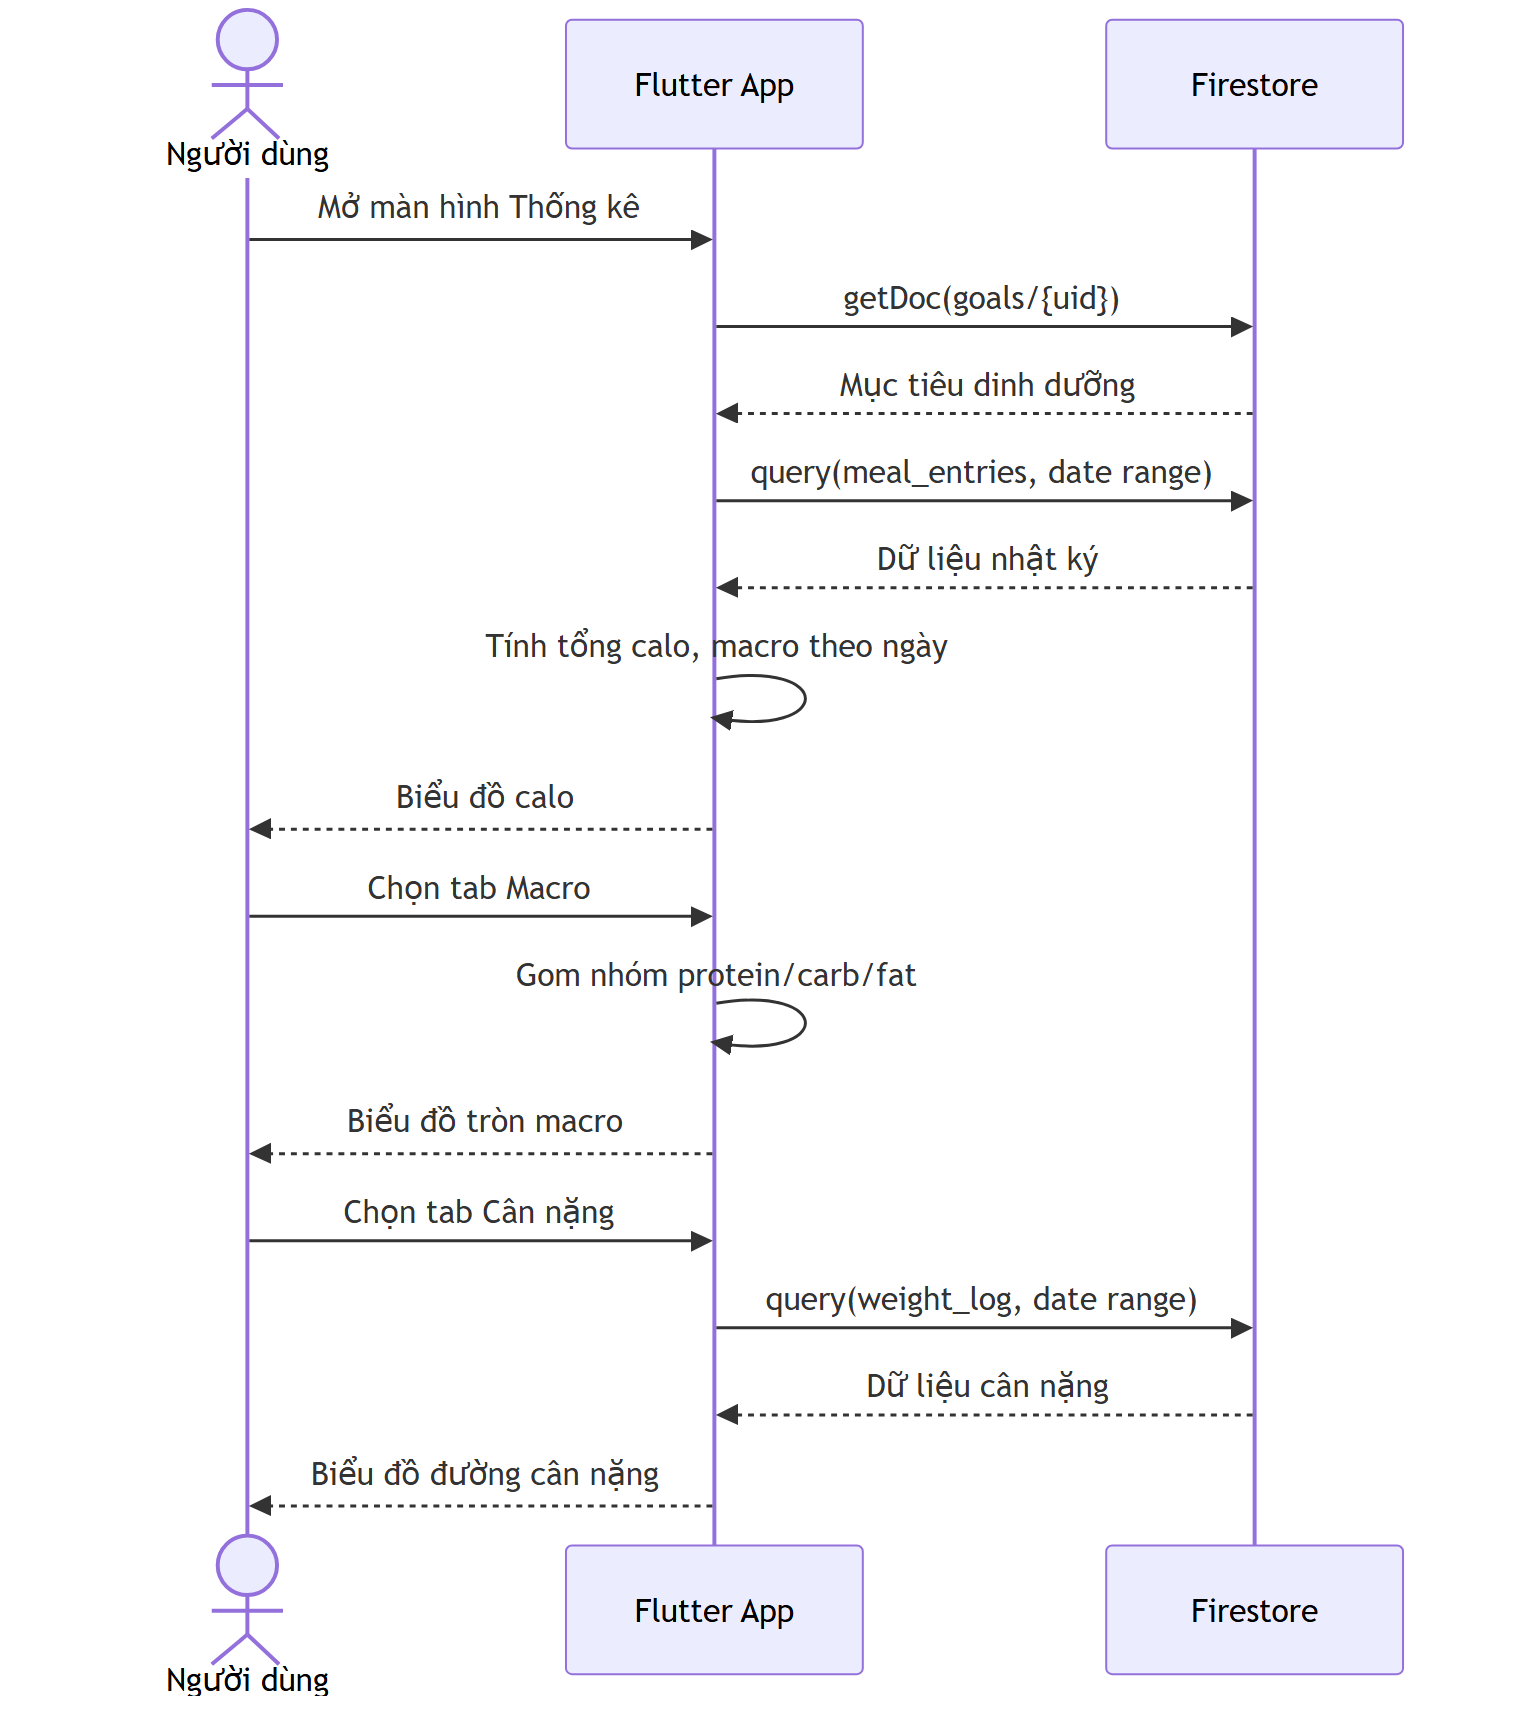
\includegraphics[width=0.9\textwidth]{assets/diagrams/uc07_stats_sequence.png}
    \caption{Biểu đồ tuần tự ca sử dụng Theo dõi dinh dưỡng}
    \label{fig:uc07_stats_sequence}
\end{figure}

% ============================================================
\subsection{UC-03: Quản lý hồ sơ cá nhân}

\begin{longtable}{|p{4cm}|p{11cm}|}
    \hline
    \textbf{Thuộc tính} & \textbf{Mô tả} \\
    \hline
    \endhead
    \hline
    \endfoot
    Tên ca sử dụng & Quản lý hồ sơ cá nhân \\
    \hline
    Mô tả & Người dùng xem và cập nhật thông tin cá nhân như họ tên, giới tính, chiều cao, cân nặng, độ tuổi và các thông tin phục vụ tính toán mục tiêu dinh dưỡng. \\
    \hline
    Actor & Người dùng đã đăng nhập \\
    \hline
    Luồng cơ bản &
        \begin{enumerate}[nosep]
            \item Người dùng mở màn hình hồ sơ cá nhân.
            \item Hệ thống tải thông tin hồ sơ hiện tại từ Firestore.
            \item Người dùng chỉnh sửa các trường thông tin cần cập nhật.
            \item Người dùng nhấn nút lưu thay đổi.
            \item Hệ thống kiểm tra dữ liệu đầu vào.
            \item Hệ thống cập nhật document hồ sơ người dùng trong Firestore.
            \item Hệ thống hiển thị thông báo cập nhật thành công.
        \end{enumerate} \\
    \hline
    Luồng thay thế &
        \begin{enumerate}[nosep]
            \item[2a.] Chưa có hồ sơ: Hệ thống hiển thị form rỗng và yêu cầu người dùng bổ sung thông tin.
            \item[5a.] Dữ liệu không hợp lệ: Hệ thống hiển thị lỗi tại trường tương ứng.
            \item[6a.] Lưu thất bại do lỗi mạng: Hệ thống thông báo lỗi và cho phép thử lại.
        \end{enumerate} \\
    \hline
    Tiền điều kiện & Người dùng đã đăng nhập vào hệ thống. \\
    \hline
    Hậu điều kiện & Thông tin hồ sơ cá nhân được cập nhật và có thể được sử dụng cho các tính năng tính toán mục tiêu dinh dưỡng. \\
    \hline
    Business Rules &
        \begin{itemize}[nosep]
            \item Người dùng chỉ được cập nhật hồ sơ của chính mình.
            \item Các trường như chiều cao, cân nặng và tuổi phải là giá trị hợp lệ.
            \item Dữ liệu hồ sơ là cơ sở để tính toán mục tiêu calo và gợi ý dinh dưỡng.
        \end{itemize} \\
    \hline
\end{longtable}

\begin{figure}[H]
    \centering
    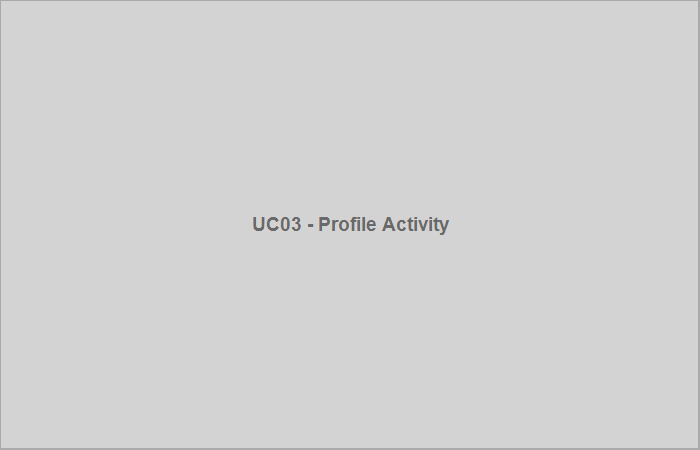
\includegraphics[width=0.8\textwidth]{assets/diagrams/uc03_profile_activity.png}
    \caption{Biểu đồ hoạt động ca sử dụng Quản lý hồ sơ cá nhân}
    \label{fig:uc03_profile_activity}
\end{figure}

\begin{figure}[H]
    \centering
    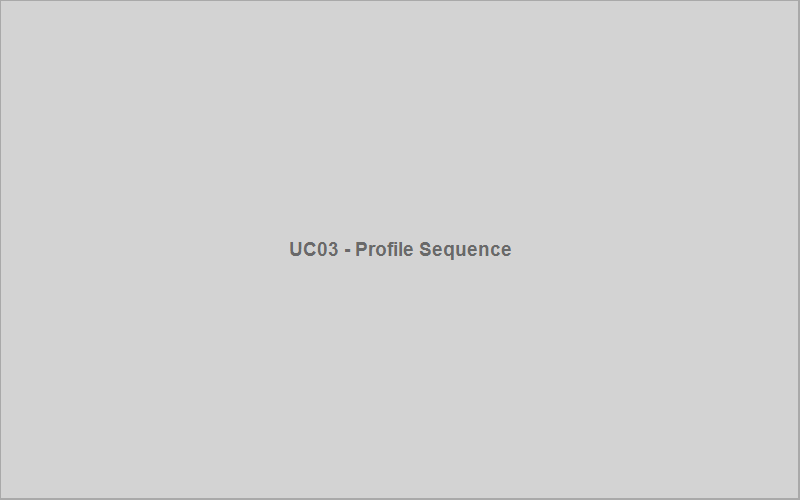
\includegraphics[width=0.9\textwidth]{assets/diagrams/uc03_profile_sequence.png}
    \caption{Biểu đồ tuần tự ca sử dụng Quản lý hồ sơ cá nhân}
    \label{fig:uc03_profile_sequence}
\end{figure}

% ============================================================
\subsection{UC-04: Hoàn thành Onboarding}

\begin{longtable}{|p{4cm}|p{11cm}|}
    \hline
    \textbf{Thuộc tính} & \textbf{Mô tả} \\
    \hline
    \endhead
    \hline
    \endfoot
    Tên ca sử dụng & Hoàn thành Onboarding \\
    \hline
    Mô tả & Người dùng mới cung cấp các thông tin ban đầu để hệ thống thiết lập hồ sơ cá nhân và mục tiêu dinh dưỡng phù hợp. \\
    \hline
    Actor & Người dùng mới đăng ký hoặc chưa hoàn thiện hồ sơ \\
    \hline
    Luồng cơ bản &
        \begin{enumerate}[nosep]
            \item Người dùng đăng nhập lần đầu hoặc được chuyển đến màn hình Onboarding.
            \item Hệ thống hiển thị các bước nhập thông tin cơ bản.
            \item Người dùng nhập tuổi, giới tính, chiều cao, cân nặng và mục tiêu sức khỏe.
            \item Hệ thống tính toán mục tiêu dinh dưỡng ban đầu dựa trên thông tin đã nhập.
            \item Người dùng xác nhận thông tin.
            \item Hệ thống lưu hồ sơ và mục tiêu dinh dưỡng vào Firestore.
            \item Hệ thống chuyển người dùng đến màn hình chính.
        \end{enumerate} \\
    \hline
    Luồng thay thế &
        \begin{enumerate}[nosep]
            \item[3a.] Người dùng nhập thiếu thông tin bắt buộc: Hệ thống yêu cầu hoàn thiện trước khi tiếp tục.
            \item[4a.] Không thể tính mục tiêu do dữ liệu không hợp lệ: Hệ thống yêu cầu kiểm tra lại thông tin.
            \item[6a.] Lưu thất bại: Hệ thống hiển thị thông báo lỗi và cho phép lưu lại.
        \end{enumerate} \\
    \hline
    Tiền điều kiện & Người dùng đã đăng nhập nhưng chưa hoàn tất hồ sơ ban đầu. \\
    \hline
    Hậu điều kiện & Hồ sơ người dùng và mục tiêu dinh dưỡng ban đầu được tạo trong hệ thống. \\
    \hline
    Business Rules &
        \begin{itemize}[nosep]
            \item Người dùng phải hoàn thành các thông tin bắt buộc trước khi sử dụng đầy đủ ứng dụng.
            \item Mục tiêu dinh dưỡng ban đầu có thể được chỉnh sửa lại sau trong phần hồ sơ hoặc mục tiêu.
            \item Dữ liệu Onboarding phải gắn với đúng tài khoản đang đăng nhập.
        \end{itemize} \\
    \hline
\end{longtable}

\begin{figure}[H]
    \centering
    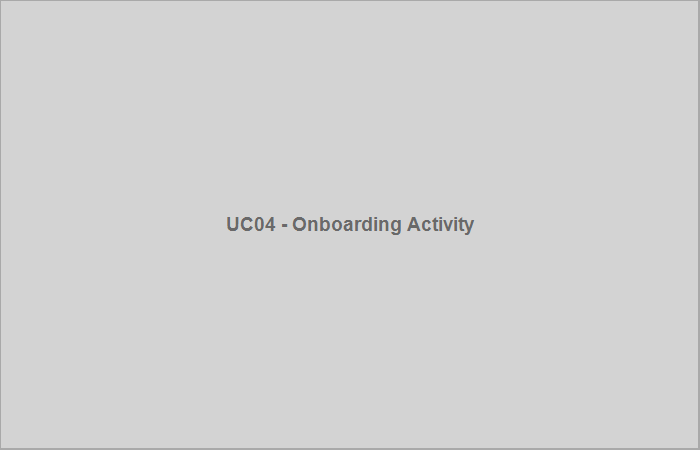
\includegraphics[width=0.8\textwidth]{assets/diagrams/uc04_onboarding_activity.png}
    \caption{Biểu đồ hoạt động ca sử dụng Hoàn thành Onboarding}
    \label{fig:uc04_onboarding_activity}
\end{figure}

\begin{figure}[H]
    \centering
    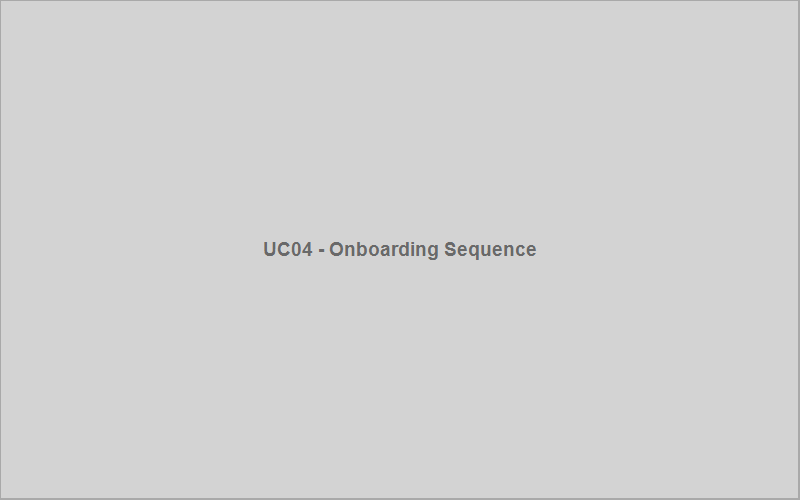
\includegraphics[width=0.9\textwidth]{assets/diagrams/uc04_onboarding_sequence.png}
    \caption{Biểu đồ tuần tự ca sử dụng Hoàn thành Onboarding}
    \label{fig:uc04_onboarding_sequence}
\end{figure}

% ============================================================
\subsection{UC-08: Quản lý món ăn yêu thích}

\begin{longtable}{|p{4cm}|p{11cm}|}
    \hline
    \textbf{Thuộc tính} & \textbf{Mô tả} \\
    \hline
    \endhead
    \hline
    \endfoot
    Tên ca sử dụng & Quản lý món ăn yêu thích \\
    \hline
    Mô tả & Người dùng thêm hoặc xóa món ăn khỏi danh sách yêu thích để có thể truy cập và thêm nhanh các món thường dùng. \\
    \hline
    Actor & Người dùng đã đăng nhập \\
    \hline
    Luồng cơ bản &
        \begin{enumerate}[nosep]
            \item Người dùng mở danh sách món ăn hoặc màn hình tìm kiếm thực phẩm.
            \item Hệ thống hiển thị trạng thái yêu thích của từng món ăn.
            \item Người dùng nhấn biểu tượng yêu thích trên một món ăn.
            \item Hệ thống kiểm tra trạng thái hiện tại của món ăn.
            \item Nếu món chưa được yêu thích, hệ thống ghi bản ghi vào `users/\{uid\}/favorites`.
            \item Nếu món đã được yêu thích, hệ thống xóa bản ghi tương ứng.
            \item Hệ thống cập nhật lại giao diện danh sách yêu thích.
        \end{enumerate} \\
    \hline
    Luồng thay thế &
        \begin{enumerate}[nosep]
            \item[2a.] Không có món yêu thích: Hệ thống hiển thị trạng thái rỗng và gợi ý người dùng thêm món.
            \item[5a.] Món ăn không còn tồn tại trong food catalog: Hệ thống bỏ qua hoặc không hiển thị món trong danh sách yêu thích.
            \item[6a.] Lỗi ghi/xóa Firestore: Hệ thống thông báo lỗi và giữ nguyên trạng thái trước đó.
        \end{enumerate} \\
    \hline
    Tiền điều kiện & Người dùng đã đăng nhập và food catalog đã được tải. \\
    \hline
    Hậu điều kiện & Danh sách món ăn yêu thích của người dùng được cập nhật. \\
    \hline
    Business Rules &
        \begin{itemize}[nosep]
            \item Mỗi món ăn yêu thích được định danh theo `foodId`.
            \item Người dùng chỉ đọc/ghi danh sách yêu thích của chính mình.
            \item Danh sách yêu thích phải đồng bộ giữa màn hình Home và màn hình Search.
        \end{itemize} \\
    \hline
\end{longtable}

\begin{figure}[H]
    \centering
    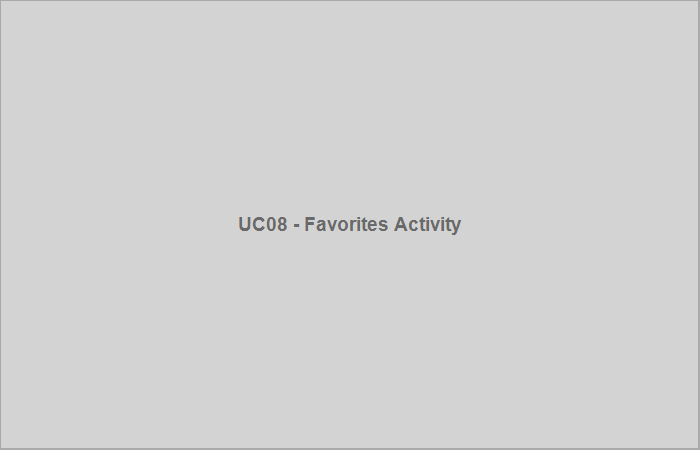
\includegraphics[width=0.8\textwidth]{assets/diagrams/uc08_favorites_activity.png}
    \caption{Biểu đồ hoạt động ca sử dụng Quản lý món ăn yêu thích}
    \label{fig:uc08_favorites_activity}
\end{figure}

\begin{figure}[H]
    \centering
    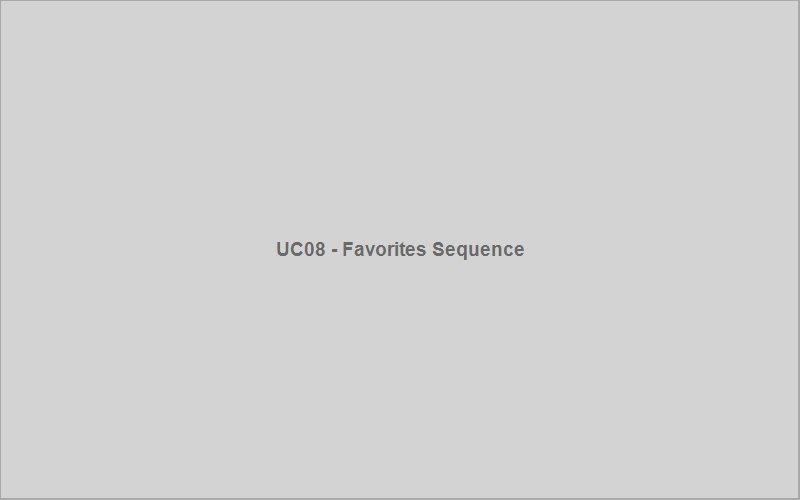
\includegraphics[width=0.9\textwidth]{assets/diagrams/uc08_favorites_sequence.png}
    \caption{Biểu đồ tuần tự ca sử dụng Quản lý món ăn yêu thích}
    \label{fig:uc08_favorites_sequence}
\end{figure}

% ============================================================
\subsection{UC-09: Chatbot AI dinh dưỡng}

\begin{longtable}{|p{4cm}|p{11cm}|}
    \hline
    \textbf{Thuộc tính} & \textbf{Mô tả} \\
    \hline
    \endhead
    \hline
    \endfoot
    Tên ca sử dụng & Chatbot AI dinh dưỡng \\
    \hline
    Mô tả & Người dùng gửi câu hỏi về dinh dưỡng và nhận phản hồi từ trợ lý AI dựa trên ngữ cảnh hồ sơ, mục tiêu và dữ liệu ăn uống hiện có. \\
    \hline
    Actor & Người dùng đã đăng nhập \\
    \hline
    Luồng cơ bản &
        \begin{enumerate}[nosep]
            \item Người dùng mở màn hình chatbot dinh dưỡng.
            \item Hệ thống tải lịch sử hội thoại gần nhất từ `users/\{uid\}/chat\_history`.
            \item Người dùng nhập câu hỏi và gửi tin nhắn.
            \item Hệ thống xây dựng ngữ cảnh từ hồ sơ, mục tiêu và nhật ký ăn uống.
            \item Hệ thống gửi yêu cầu đến dịch vụ AI đã cấu hình.
            \item Dịch vụ AI trả về nội dung phản hồi và gợi ý câu hỏi tiếp theo.
            \item Hệ thống lưu cặp tin nhắn người dùng/trợ lý vào lịch sử hội thoại.
            \item Hệ thống hiển thị phản hồi cho người dùng.
        \end{enumerate} \\
    \hline
    Luồng thay thế &
        \begin{enumerate}[nosep]
            \item[2a.] Chưa có lịch sử hội thoại: Hệ thống hiển thị tin nhắn chào mừng mặc định.
            \item[5a.] Dịch vụ AI chưa được cấu hình: Hệ thống hiển thị thông báo không thể sử dụng AI lúc này.
            \item[5b.] Lỗi mạng hoặc lỗi từ dịch vụ AI: Hệ thống hiển thị tin nhắn lỗi và cho phép người dùng thử lại.
        \end{enumerate} \\
    \hline
    Tiền điều kiện & Người dùng đã đăng nhập; dịch vụ AI được cấu hình hợp lệ. \\
    \hline
    Hậu điều kiện & Tin nhắn mới được hiển thị trên giao diện chat và được lưu vào lịch sử hội thoại nếu thao tác lưu thành công. \\
    \hline
    Business Rules &
        \begin{itemize}[nosep]
            \item Chatbot chỉ đưa ra thông tin tham khảo, không thay thế tư vấn y tế chuyên môn.
            \item Lịch sử hội thoại của người dùng phải được tách biệt theo tài khoản.
            \item Nội dung phản hồi cần phù hợp với ngữ cảnh dinh dưỡng của người dùng nếu có dữ liệu liên quan.
        \end{itemize} \\
    \hline
\end{longtable}

\begin{figure}[H]
    \centering
    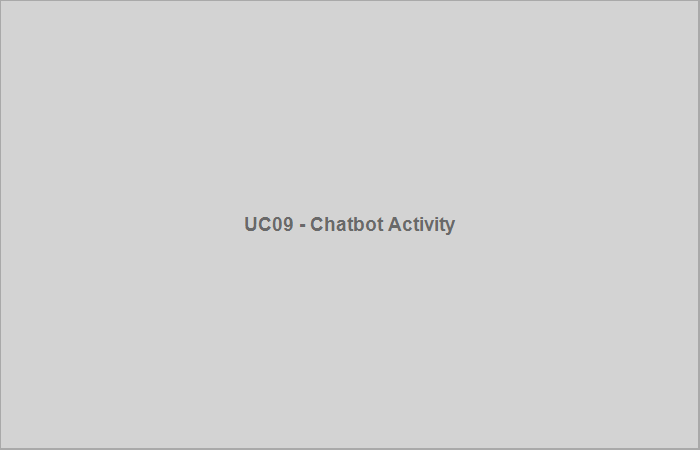
\includegraphics[width=0.8\textwidth]{assets/diagrams/uc09_chatbot_activity.png}
    \caption{Biểu đồ hoạt động ca sử dụng Chatbot AI dinh dưỡng}
    \label{fig:uc09_chatbot_activity}
\end{figure}

\begin{figure}[H]
    \centering
    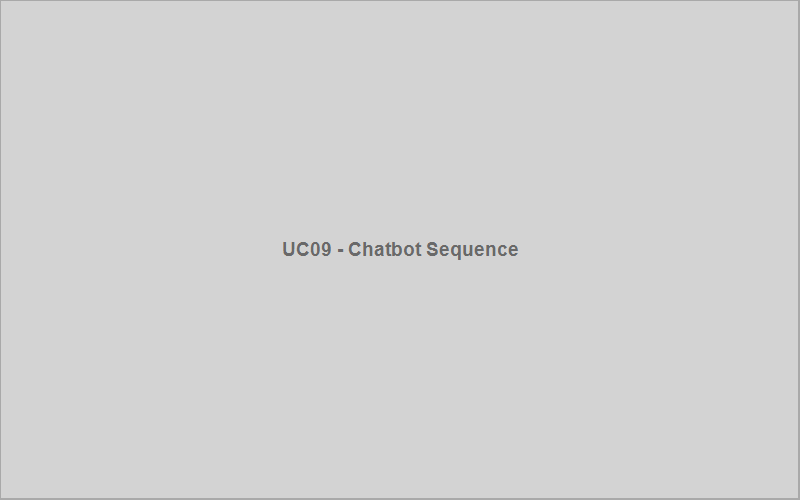
\includegraphics[width=0.9\textwidth]{assets/diagrams/uc09_chatbot_sequence.png}
    \caption{Biểu đồ tuần tự ca sử dụng Chatbot AI dinh dưỡng}
    \label{fig:uc09_chatbot_sequence}
\end{figure}

% ============================================================
\subsection{UC-10: Quản lý thực phẩm}

\begin{longtable}{|p{4cm}|p{11cm}|}
    \hline
    \textbf{Thuộc tính} & \textbf{Mô tả} \\
    \hline
    \endhead
    \hline
    \endfoot
    Tên ca sử dụng & Quản lý thực phẩm \\
    \hline
    Mô tả & Quản trị viên quản lý dữ liệu thực phẩm trong food catalog, bao gồm xem danh sách, tìm kiếm, thêm mới, chỉnh sửa hoặc vô hiệu hóa món ăn. \\
    \hline
    Actor & Quản trị viên \\
    \hline
    Luồng cơ bản &
        \begin{enumerate}[nosep]
            \item Quản trị viên đăng nhập vào trang quản trị.
            \item Hệ thống xác thực quyền quản trị.
            \item Quản trị viên mở màn hình quản lý thực phẩm.
            \item Hệ thống hiển thị danh sách thực phẩm từ collection `foods`.
            \item Quản trị viên thực hiện thao tác thêm, sửa hoặc vô hiệu hóa thực phẩm.
            \item Hệ thống kiểm tra tính hợp lệ của dữ liệu dinh dưỡng.
            \item Hệ thống ghi thay đổi vào Firestore.
            \item Hệ thống cập nhật lại danh sách thực phẩm trên giao diện.
        \end{enumerate} \\
    \hline
    Luồng thay thế &
        \begin{enumerate}[nosep]
            \item[2a.] Tài khoản không có quyền admin: Hệ thống từ chối truy cập.
            \item[6a.] Thiếu trường bắt buộc hoặc giá trị dinh dưỡng không hợp lệ: Hệ thống hiển thị lỗi nhập liệu.
            \item[7a.] Ghi dữ liệu thất bại: Hệ thống thông báo lỗi và không cập nhật giao diện thành công.
        \end{enumerate} \\
    \hline
    Tiền điều kiện & Quản trị viên đã đăng nhập và có quyền quản trị. \\
    \hline
    Hậu điều kiện & Dữ liệu food catalog được cập nhật theo thao tác hợp lệ của quản trị viên. \\
    \hline
    Business Rules &
        \begin{itemize}[nosep]
            \item Chỉ tài khoản có quyền admin mới được ghi vào collection `foods`.
            \item Thông tin dinh dưỡng phải có các chỉ số cơ bản như calo, protein, carbohydrate và chất béo.
            \item Không nên xóa cứng dữ liệu đang được tham chiếu bởi nhật ký người dùng; ưu tiên vô hiệu hóa nếu cần ẩn món ăn.
        \end{itemize} \\
    \hline
\end{longtable}

\begin{figure}[H]
    \centering
    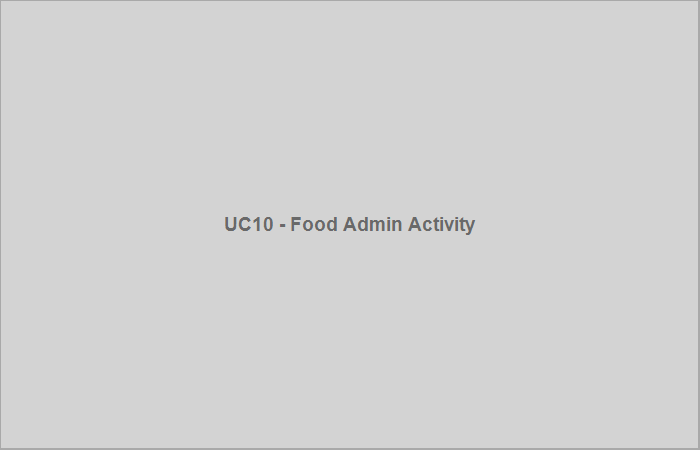
\includegraphics[width=0.8\textwidth]{assets/diagrams/uc10_food_admin_activity.png}
    \caption{Biểu đồ hoạt động ca sử dụng Quản lý thực phẩm}
    \label{fig:uc10_food_admin_activity}
\end{figure}

\begin{figure}[H]
    \centering
    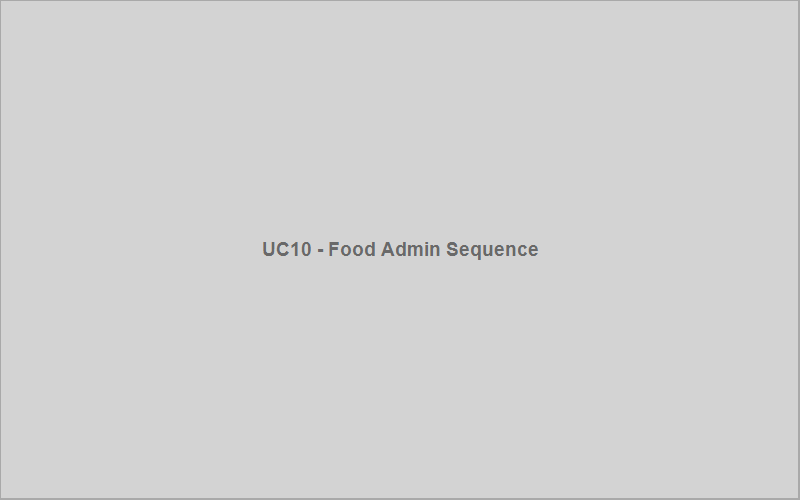
\includegraphics[width=0.9\textwidth]{assets/diagrams/uc10_food_admin_sequence.png}
    \caption{Biểu đồ tuần tự ca sử dụng Quản lý thực phẩm}
    \label{fig:uc10_food_admin_sequence}
\end{figure}

% ============================================================
\subsection{UC-11: Quản lý người dùng}

\begin{longtable}{|p{4cm}|p{11cm}|}
    \hline
    \textbf{Thuộc tính} & \textbf{Mô tả} \\
    \hline
    \endhead
    \hline
    \endfoot
    Tên ca sử dụng & Quản lý người dùng \\
    \hline
    Mô tả & Quản trị viên xem danh sách người dùng, theo dõi thông tin cơ bản và trạng thái sử dụng để phục vụ công tác quản trị hệ thống. \\
    \hline
    Actor & Quản trị viên \\
    \hline
    Luồng cơ bản &
        \begin{enumerate}[nosep]
            \item Quản trị viên đăng nhập vào trang quản trị.
            \item Hệ thống xác thực quyền quản trị.
            \item Quản trị viên mở màn hình quản lý người dùng.
            \item Hệ thống truy xuất danh sách người dùng từ collection `users`.
            \item Quản trị viên tìm kiếm hoặc lọc danh sách theo thông tin cần xem.
            \item Hệ thống hiển thị thông tin hồ sơ, trạng thái gói dịch vụ và usage liên quan nếu có.
        \end{enumerate} \\
    \hline
    Luồng thay thế &
        \begin{enumerate}[nosep]
            \item[2a.] Tài khoản không có quyền admin: Hệ thống từ chối truy cập.
            \item[4a.] Không tải được danh sách người dùng: Hệ thống hiển thị thông báo lỗi.
            \item[5a.] Không có kết quả tìm kiếm phù hợp: Hệ thống hiển thị trạng thái rỗng.
        \end{enumerate} \\
    \hline
    Tiền điều kiện & Quản trị viên đã đăng nhập và có quyền truy cập trang quản trị. \\
    \hline
    Hậu điều kiện & Quản trị viên xem được thông tin người dùng phục vụ theo dõi và quản trị. \\
    \hline
    Business Rules &
        \begin{itemize}[nosep]
            \item Thông tin người dùng chỉ được hiển thị cho tài khoản có quyền admin.
            \item Các dữ liệu nhạy cảm như mật khẩu không được lưu hoặc hiển thị trong Firestore.
            \item Các thao tác thay đổi trạng thái người dùng cần được kiểm soát quyền chặt chẽ.
        \end{itemize} \\
    \hline
\end{longtable}

\begin{figure}[H]
    \centering
    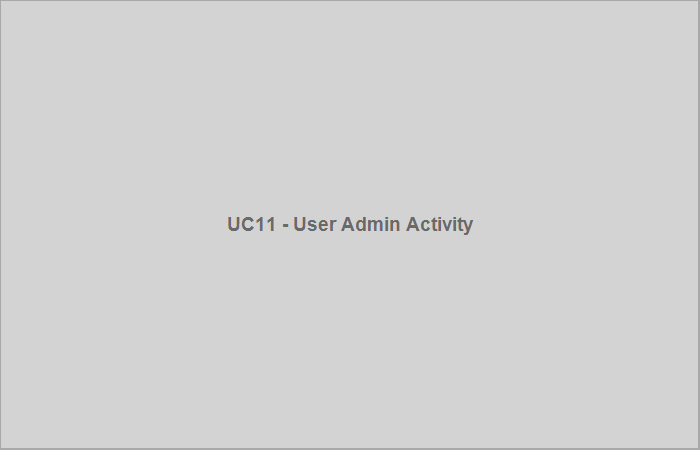
\includegraphics[width=0.8\textwidth]{assets/diagrams/uc11_user_admin_activity.png}
    \caption{Biểu đồ hoạt động ca sử dụng Quản lý người dùng}
    \label{fig:uc11_user_admin_activity}
\end{figure}

\begin{figure}[H]
    \centering
    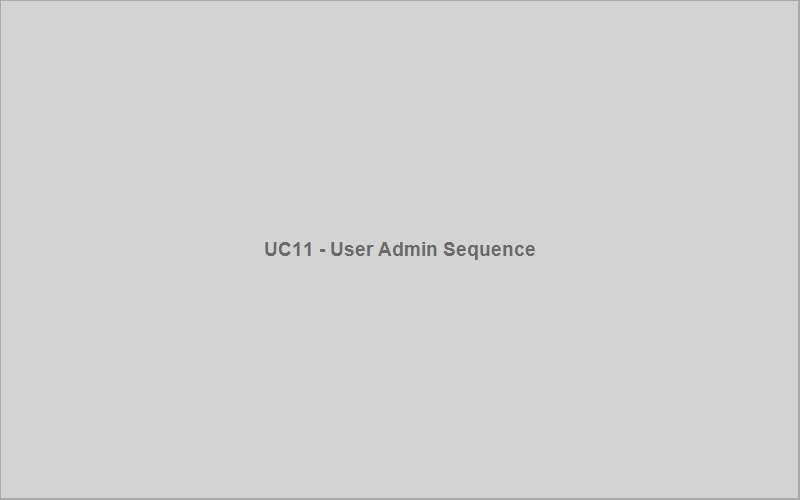
\includegraphics[width=0.9\textwidth]{assets/diagrams/uc11_user_admin_sequence.png}
    \caption{Biểu đồ tuần tự ca sử dụng Quản lý người dùng}
    \label{fig:uc11_user_admin_sequence}
\end{figure}

% ============================================================
\subsection{UC-12: Đăng ký Premium}

\begin{longtable}{|p{4cm}|p{11cm}|}
    \hline
    \textbf{Thuộc tính} & \textbf{Mô tả} \\
    \hline
    \endhead
    \hline
    \endfoot
    Tên ca sử dụng & Đăng ký Premium \\
    \hline
    Mô tả & Người dùng xem quyền lợi gói Premium và thực hiện thao tác đăng ký hoặc nâng cấp để mở khóa các tính năng nâng cao. \\
    \hline
    Actor & Người dùng đã đăng nhập \\
    \hline
    Luồng cơ bản &
        \begin{enumerate}[nosep]
            \item Người dùng mở màn hình gói dịch vụ hoặc màn hình paywall.
            \item Hệ thống hiển thị thông tin gói Free và Premium.
            \item Người dùng chọn nâng cấp lên Premium.
            \item Hệ thống kiểm tra trạng thái subscription hiện tại của người dùng.
            \item Hệ thống ghi nhận yêu cầu nâng cấp theo cơ chế thanh toán hoặc cơ chế demo đang được cấu hình.
            \item Hệ thống cập nhật thông tin `subscription` trong document người dùng.
            \item Hệ thống cập nhật giao diện và mở khóa quyền lợi Premium tương ứng.
        \end{enumerate} \\
    \hline
    Luồng thay thế &
        \begin{enumerate}[nosep]
            \item[4a.] Người dùng đã là Premium: Hệ thống hiển thị trạng thái gói hiện tại.
            \item[5a.] Thanh toán hoặc thao tác nâng cấp thất bại: Hệ thống thông báo lỗi và giữ nguyên trạng thái hiện tại.
            \item[6a.] Cập nhật Firestore thất bại: Hệ thống hiển thị thông báo lỗi và yêu cầu thử lại.
        \end{enumerate} \\
    \hline
    Tiền điều kiện & Người dùng đã đăng nhập và có kết nối mạng. \\
    \hline
    Hậu điều kiện & Trạng thái gói dịch vụ của người dùng được cập nhật nếu thao tác nâng cấp thành công. \\
    \hline
    Business Rules &
        \begin{itemize}[nosep]
            \item Người dùng Free bị giới hạn số lượt sử dụng một số tính năng AI theo tháng.
            \item Người dùng Premium được mở khóa giới hạn cao hơn hoặc các tính năng nâng cao tùy cấu hình hệ thống.
            \item Trạng thái subscription phải được lưu trong document `users/\{uid\}` và được kiểm tra trước khi cấp quyền.
        \end{itemize} \\
    \hline
\end{longtable}

\begin{figure}[H]
    \centering
    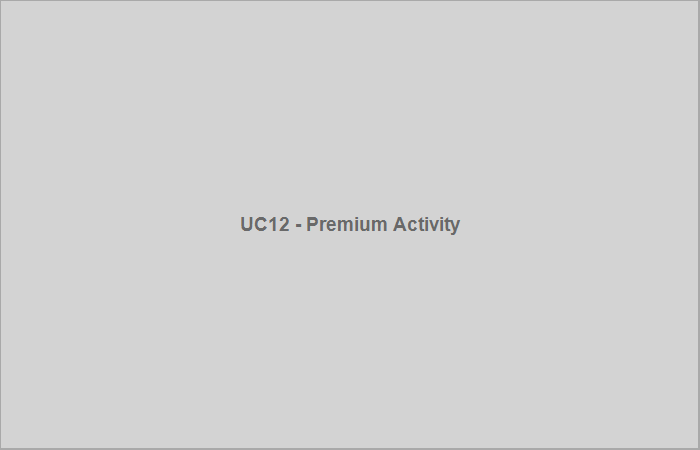
\includegraphics[width=0.8\textwidth]{assets/diagrams/uc12_premium_activity.png}
    \caption{Biểu đồ hoạt động ca sử dụng Đăng ký Premium}
    \label{fig:uc12_premium_activity}
\end{figure}

\begin{figure}[H]
    \centering
    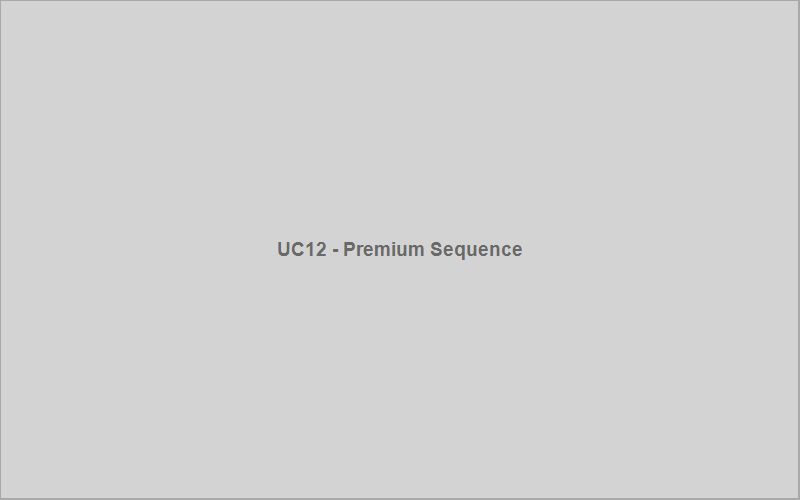
\includegraphics[width=0.9\textwidth]{assets/diagrams/uc12_premium_sequence.png}
    \caption{Biểu đồ tuần tự ca sử dụng Đăng ký Premium}
    \label{fig:uc12_premium_sequence}
\end{figure}

\section{Thiết kế cơ sở dữ liệu}

Hệ thống sử dụng Cloud Firestore — cơ sở dữ liệu NoSQL dạng document. Dữ liệu được tổ chức theo cấu trúc collection và document, trong đó mỗi document có thể chứa các sub-collection.

\subsection{Sơ đồ thực thể - liên kết (ERD)}

\begin{figure}[H]
    \centering
    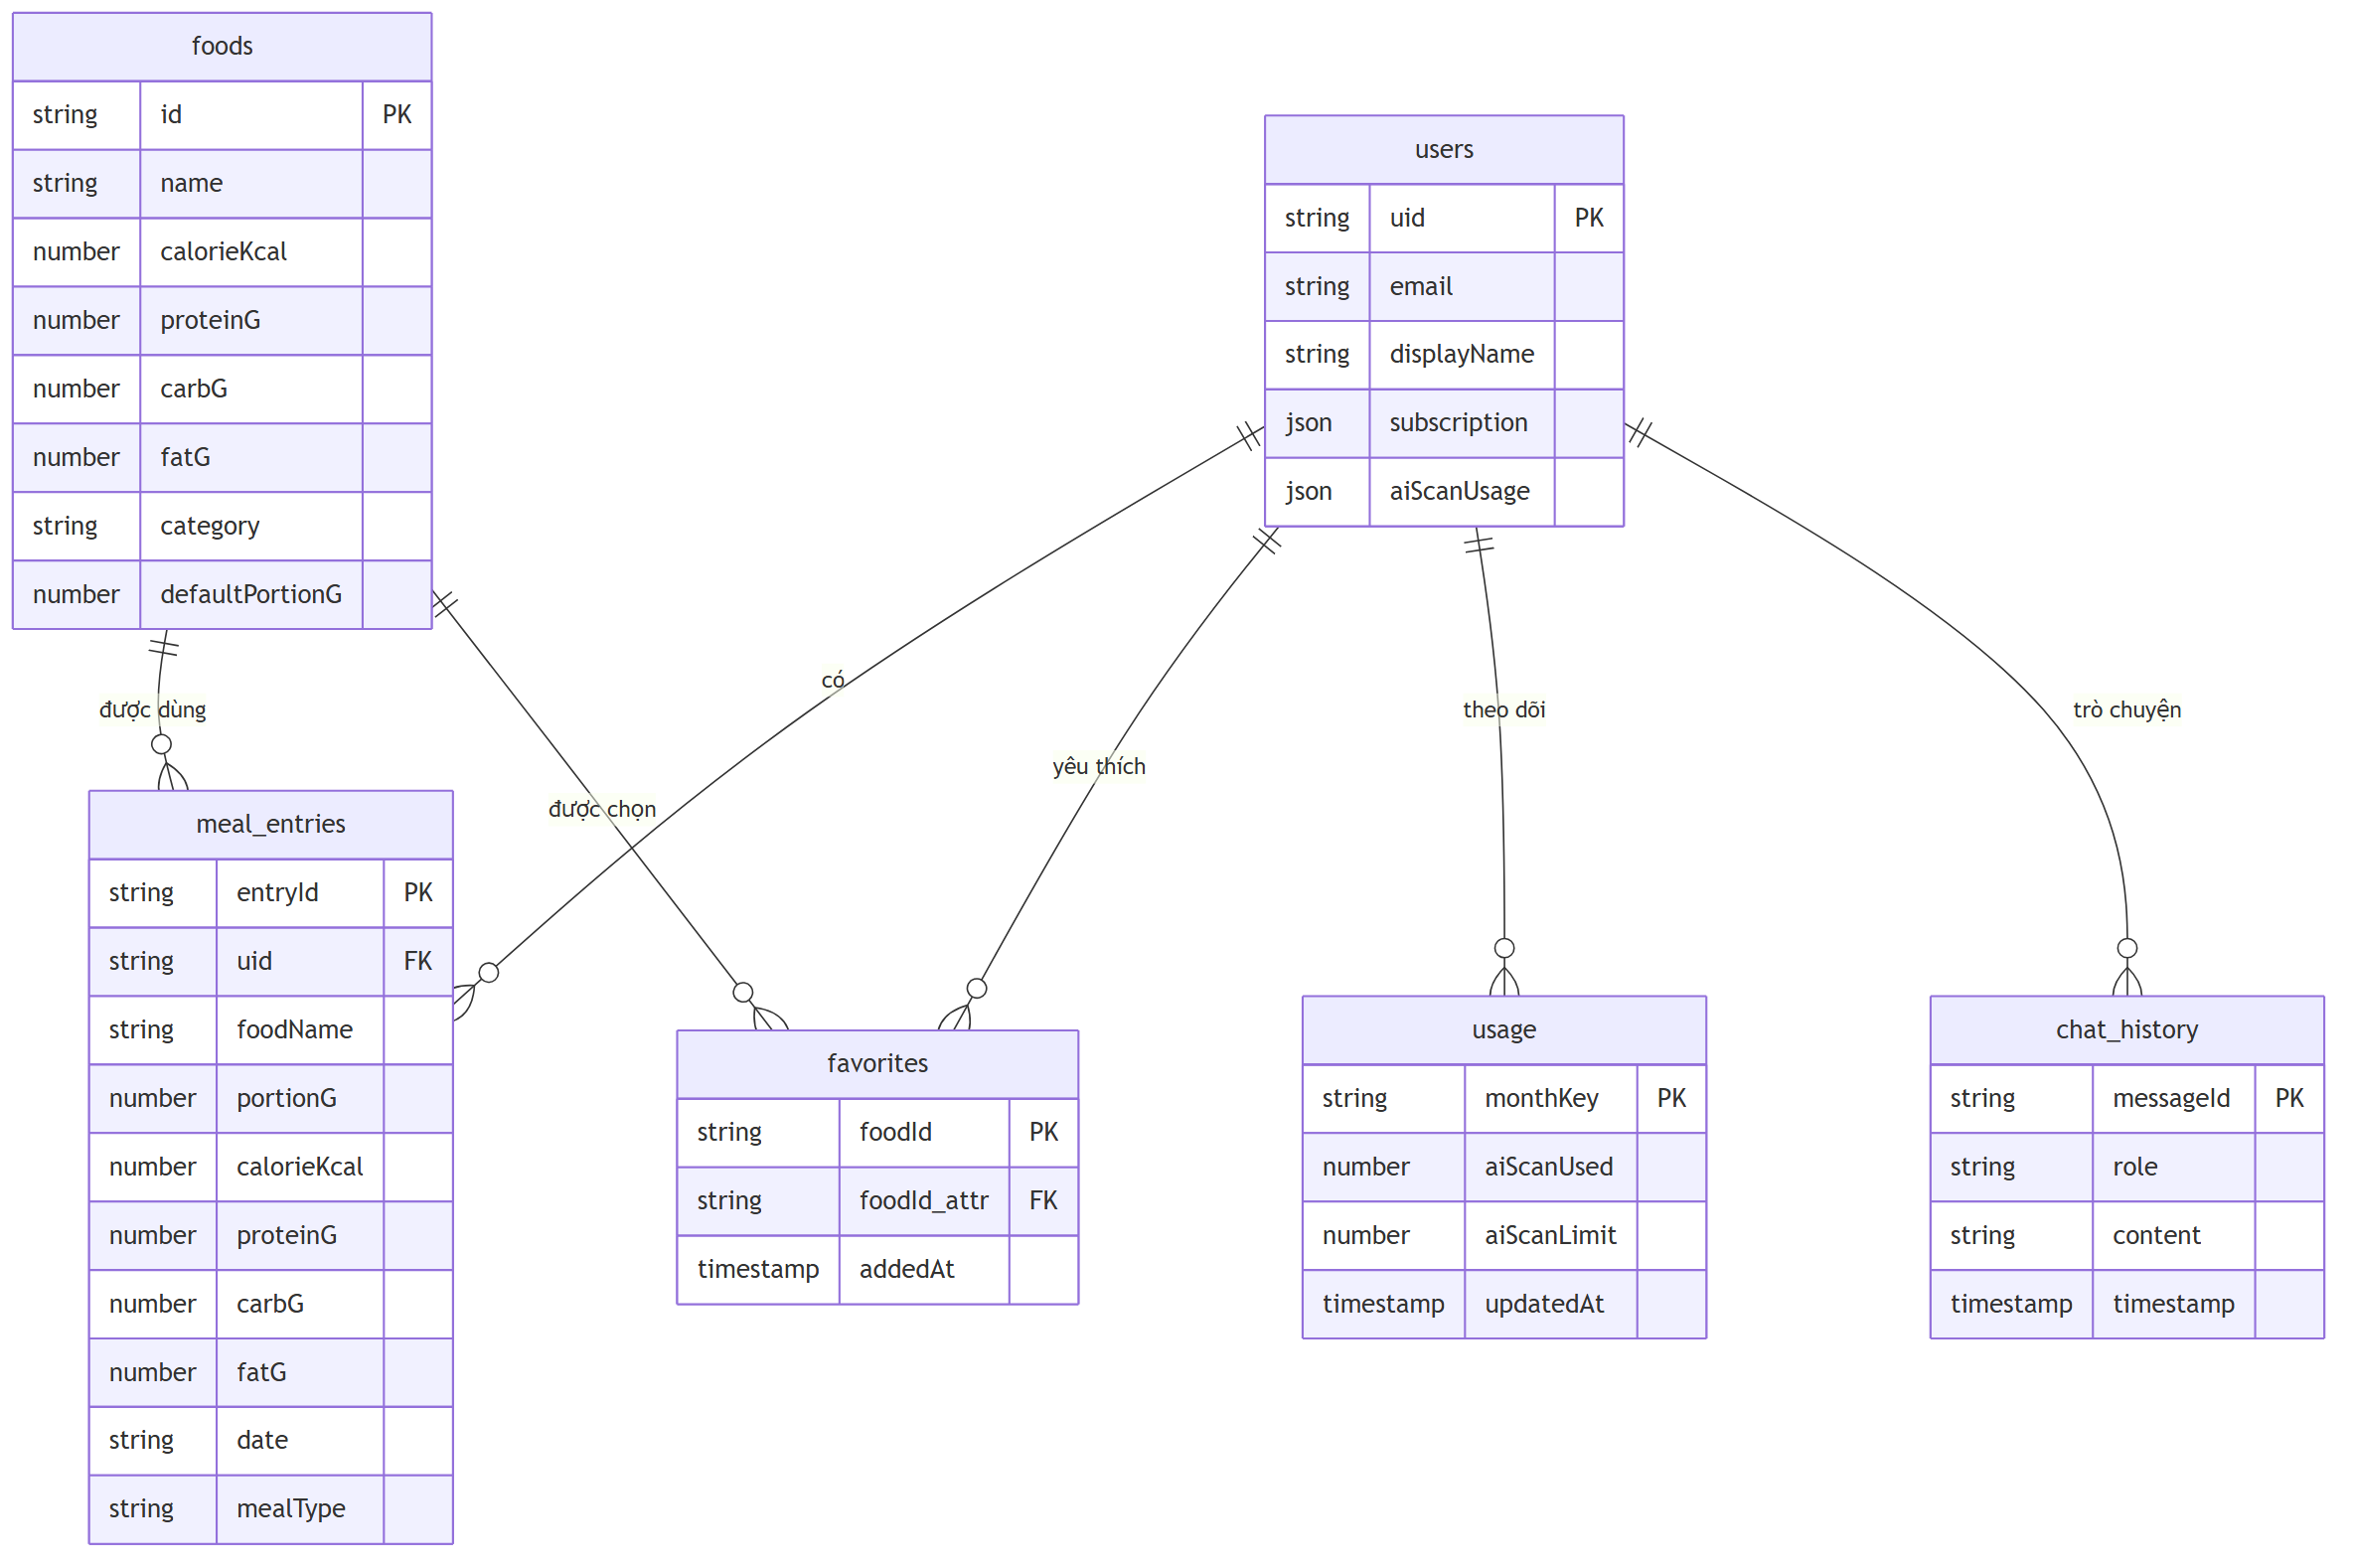
\includegraphics[width=0.9\textwidth]{assets/diagrams/erd_diagram.png}
    \caption{Biểu đồ thực thể - liên kết hệ thống SmartNutri}
    \label{fig:erd_diagram}
\end{figure}

\subsection{Mô tả các collection chính}

\subsubsection{Collection: users}

Lưu trữ thông tin người dùng. Mỗi document được định danh bằng user ID từ Firebase Authentication.

\begin{longtable}{|p{3.5cm}|p{3.5cm}|p{7.5cm}|}
    \hline
    \textbf{Trường} & \textbf{Kiểu dữ liệu} & \textbf{Mô tả} \\
    \hline
    \endhead
    \hline
    \endfoot
    email & String & Email người dùng \\
    \hline
    displayName & String & Tên hiển thị \\
    \hline
    photoURL & String & URL ảnh đại diện \\
    \hline
    height & Number & Chiều cao (cm) \\
    \hline
    weight & Number & Cân nặng (kg) \\
    \hline
    age & Number & Tuổi \\
    \hline
    gender & String & Giới tính \\
    \hline
    goal & String & Mục tiêu dinh dưỡng \\
    \hline
    dailyCalorieTarget & Number & Mục tiêu calo/ngày \\
    \hline
    isPremium & Boolean & Trạng thái Premium \\
    \hline
    createdAt & Timestamp & Thời điểm tạo tài khoản \\
    \hline
\end{longtable}

\subsubsection{Collection: foods}

Lưu trữ cơ sở dữ liệu thực phẩm và món ăn.

\begin{longtable}{|p{3.5cm}|p{3.5cm}|p{7.5cm}|}
    \hline
    \textbf{Trường} & \textbf{Kiểu dữ liệu} & \textbf{Mô tả} \\
    \hline
    \endhead
    \hline
    \endfoot
    name & String & Tên món ăn (tiếng Việt) \\
    \hline
    nameEn & String & Tên món ăn (tiếng Anh) \\
    \hline
    category & String & Danh mục (cơm, phở, canh, ...) \\
    \hline
    calories & Number & Lượng calo (kcal/100g) \\
    \hline
    protein & Number & Lượng protein (g/100g) \\
    \hline
    carbs & Number & Lượng carbohydrate (g/100g) \\
    \hline
    fat & Number & Lượng chất béo (g/100g) \\
    \hline
    fiber & Number & Lượng chất xơ (g/100g) \\
    \hline
    imageURL & String & URL hình ảnh món ăn \\
    \hline
    servingSize & String & Đơn vị khẩu phần \\
    \hline
    isActive & Boolean & Trạng thái hiển thị \\
    \hline
    createdAt & Timestamp & Thời điểm tạo \\
    \hline
\end{longtable}

\subsubsection{Sub-collection: users/\{userId\}/meal\_entries}

Lưu trữ nhật ký ăn uống hàng ngày của từng người dùng. Mỗi bản ghi thể hiện một món ăn hoặc thực phẩm được người dùng thêm vào một bữa ăn cụ thể.

\begin{longtable}{|p{3.5cm}|p{3.5cm}|p{7.5cm}|}
    \hline
    \textbf{Trường} & \textbf{Kiểu dữ liệu} & \textbf{Mô tả} \\
    \hline
    \endhead
    \hline
    \endfoot
    uid & String & ID người dùng sở hữu bản ghi \\
    \hline
    date & String & Ngày ghi nhận bữa ăn \\
    \hline
    mealType & String & Loại bữa ăn (sáng, trưa, tối, bữa phụ) \\
    \hline
    foodName & String & Tên món ăn hoặc thực phẩm \\
    \hline
    portionG & Number & Khối lượng khẩu phần tính theo gram \\
    \hline
    calorieKcal & Number & Năng lượng tính theo kcal \\
    \hline
    proteinG & Number & Lượng protein tính theo gram \\
    \hline
    carbG & Number & Lượng carbohydrate tính theo gram \\
    \hline
    fatG & Number & Lượng chất béo tính theo gram \\
    \hline
    loggedAt & Timestamp & Thời điểm ghi nhận \\
    \hline
\end{longtable}

\subsubsection{Sub-collection: users/\{userId\}/favorites}

Lưu trữ danh sách món ăn yêu thích của từng người dùng. Collection này giúp người dùng truy cập nhanh các món thường xuyên sử dụng trên màn hình Home hoặc Search.

\begin{longtable}{|p{3.5cm}|p{3.5cm}|p{7.5cm}|}
    \hline
    \textbf{Trường} & \textbf{Kiểu dữ liệu} & \textbf{Mô tả} \\
    \hline
    \endhead
    \hline
    \endfoot
    foodId & String & ID món ăn được yêu thích; thường trùng với ID document \\
    \hline
    addedAt & Timestamp & Thời điểm người dùng thêm món vào danh sách yêu thích \\
    \hline
\end{longtable}

\subsubsection{Thông tin subscription trong users/\{userId\}}

Thông tin gói dịch vụ được lưu trực tiếp trong document người dùng dưới field `subscription`. Cách lưu này giúp ứng dụng nhanh chóng xác định quyền lợi hiện tại của người dùng mà không cần truy vấn thêm collection riêng.

\begin{longtable}{|p{3.5cm}|p{3.5cm}|p{7.5cm}|}
    \hline
    \textbf{Trường} & \textbf{Kiểu dữ liệu} & \textbf{Mô tả} \\
    \hline
    \endhead
    \hline
    \endfoot
    subscription.plan & String & Tên gói dịch vụ, ví dụ `free` hoặc `premium` \\
    \hline
    subscription.status & String & Trạng thái gói, ví dụ `none`, `active` hoặc trạng thái mở rộng khác \\
    \hline
    subscription.source & String & Nguồn cập nhật gói, ví dụ `default`, `admin`, `mock` hoặc `iap` \\
    \hline
    subscription.premiumUntil & Timestamp & Thời điểm hết hạn Premium nếu có \\
    \hline
    subscription.updatedAt & Timestamp & Thời điểm cập nhật trạng thái subscription gần nhất \\
    \hline
\end{longtable}

\subsubsection{Sub-collection: users/\{userId\}/usage}

Lưu trữ số lượt sử dụng tính năng AI theo từng tháng, phục vụ việc giới hạn quota cho người dùng Free và theo dõi quyền lợi của người dùng Premium.

\begin{longtable}{|p{3.5cm}|p{3.5cm}|p{7.5cm}|}
    \hline
    \textbf{Trường} & \textbf{Kiểu dữ liệu} & \textbf{Mô tả} \\
    \hline
    \endhead
    \hline
    \endfoot
    monthKey & String & Khóa tháng theo định dạng `yyyy-MM` \\
    \hline
    aiScanUsed & Number & Số lượt quét AI đã sử dụng trong tháng \\
    \hline
    aiScanLimit & Number & Giới hạn lượt quét AI trong tháng \\
    \hline
    updatedAt & Timestamp & Thời điểm cập nhật usage gần nhất \\
    \hline
\end{longtable}

\subsubsection{Sub-collection: users/\{userId\}/chat\_history}

Lưu trữ lịch sử hội thoại giữa người dùng và chatbot dinh dưỡng. Dữ liệu này được dùng để hiển thị lại cuộc trò chuyện gần nhất và cung cấp ngữ cảnh cho các lượt chat tiếp theo.

\begin{longtable}{|p{3.5cm}|p{3.5cm}|p{7.5cm}|}
    \hline
    \textbf{Trường} & \textbf{Kiểu dữ liệu} & \textbf{Mô tả} \\
    \hline
    \endhead
    \hline
    \endfoot
    role & String & Vai trò của tin nhắn, gồm `user` hoặc `assistant` \\
    \hline
    content & String & Nội dung tin nhắn \\
    \hline
    suggestions & Array<String> & Danh sách gợi ý câu hỏi tiếp theo, thường có trong tin nhắn của assistant \\
    \hline
    isError & Boolean & Đánh dấu tin nhắn lỗi nếu quá trình xử lý AI thất bại \\
    \hline
    timestamp & Timestamp & Thời điểm ghi nhận tin nhắn \\
    \hline
\end{longtable}
